\documentclass{article}
\usepackage{polyglossia}
\usepackage{graphicx}
\usepackage{wrapfig}
\usepackage{subcaption}
\usepackage[hyphens]{url}
\usepackage{hyperref}
\usepackage{amsmath} 
\usepackage{xcolor}
\usepackage{amssymb} 
\usepackage{nameref}
\usepackage{enumitem}
\usepackage[most]{tcolorbox}
\usepackage[a4paper, top=2.5cm, bottom=2.5cm, left=2cm, right=2cm]{geometry}
\usepackage[backend=biber, style=numeric]{biblatex}
\addbibresource{references.bib}
\setmonofont{FreeMono}
\usepackage{caption}
\usepackage{ragged2e}
\usepackage{float}
\usepackage{multicol}
\makeatletter

\usepackage{listings}

\setdefaultlanguage{hebrew}
\setotherlanguage{english}  
\newfontfamily\hebrewfont[Script=Hebrew]{David CLM}
\newfontfamily\hebrewfontsf[Script=Hebrew]{Miriam CLM}

\makeatletter

\DeclareCiteCommand{\mycite}
  {\usebibmacro{prenote}}
  {\printnames{author} \bibhyperref{\mkbibbrackets{\printfield{labelnumber}}}}
  {\multicitedelim}
  {\usebibmacro{postnote}}

\DeclareCiteCommand{\urlcite}
  {\usebibmacro{prenote}}
  {\printnames{author},
   \textit{\printfield{title}},
   \printfield{year}.
   \bibhyperref{\mkbibbrackets{\printfield{labelnumber}}}}
  {\multicitedelim}
  {\usebibmacro{postnote}}



\definecolor{codegreen}{rgb}{0,0.6,0}
\definecolor{codegray}{rgb}{0.5,0.5,0.5}
\definecolor{codepurple}{rgb}{0.58,0,0.82}
\definecolor{backcolour}{rgb}{0.95,0.95,0.92}

\lstdefinestyle{mystyle}{
    backgroundcolor=\color{backcolour},   
    commentstyle=\color{codegreen},
    keywordstyle=\color{magenta},
    numberstyle=\tiny\color{codegray},
    stringstyle=\color{codepurple},
    basicstyle=\ttfamily\footnotesize,
    breakatwhitespace=false,         
    breaklines=true,                 
    captionpos=b,                    
    keepspaces=true,                 
    numbers=left,                    
    numbersep=5pt,                  
    showspaces=false,                
    showstringspaces=false,
    showtabs=false,                  
    tabsize=2,
    xleftmargin=2em
}
\lstset{style=mystyle}
\renewcommand{\lstlistingname}{קטע קוד}

\newlength{\fnrulewidth}
\setlength{\fnrulewidth}{\textwidth}
\renewcommand{\footnoterule}{%
  \kern-3pt
  \hbox to \fnrulewidth{\hfill\rule{2in}{0.4pt}}%
  \kern2.6pt
}


\begin{document}
%\onecolumn
\noindent
{\LARGE \textbf{עידוש כבידתי - אנליזה של אירועי מיקרו עידוש, אירועים
\mbox{2008-SMC-001},
\mbox{2008-BLG-002}
ואירועים נוספים 
}} \\[0.5cm]
{\large יואב וסרמן
\noindent\\
אדר שרבי}\\
{\large 8 ביולי 2026}\\

\section*{תקציר}
בדוח זו אנו מנתחים אירועים שונים של עידוש כבידתי, בעזרת מדידות של עוצמת האור של כוכב כפונקציה של הזמן, ומציגים כיצד ניתן לחלץ באמצעות כלים מתמטיים וסטטיסטים
כגון קירובים לינארים ולא-לינאריים, מינימזציית
$\chi^2$,
$\chi^2_{red}$,
 מספר גדלים המאפיינים את אירועי העידוש.
האירועים שניתחנו נלקחו מתוך מאגר המידע של
\textenglish{OGLE}
\cite{ogle_general_data}.
והם האירועים:
\mbox{BLG-004}, \mbox{BLG-005}, \mbox{BLG-007}, \mbox{BLG-034}, \mbox{BLG-049}, \mbox{BLG-006}, 
\mbox{BLG-053}, \mbox{BLG-009}\footnote{משנת 2008}
ובפרט התמקדנו באירועים
\mbox{2008-SMC-001},
\mbox{2008-BLG-002}.
בחלקים שונים של הניסוי חילצנו את הפרמטרים 
$\tau$, $u_{\min}$, $T_0$, $f_{bl}$,
תחת קירובים שונים , והשוונו את השגיאה שנוצרת כתוצאה מהקירובים השונים לערכים שחושבו על ידי 
\textenglish{OGLE}.
השיטות שהשתמשנו בהן הניבו דיוק גבוה ביחס לערכי \textenglish{OGLE} 
, למרות שבחלקים מתקדמים של הניסוי נאלצנו להתפשר על רזולוציית החישובים עקב זמני ריצה ארוכים.



\vspace{0.5cm}
\begin{multicols}{2}
\section{הקדמה}

תופעת העידוש הכבידתי היא תופעה בה מסה מעקמת קרני אור העוברות לידה וגורמת לתופעות
אופטיות שונות, כגון הגברה ועיוות בדמות העצם שפלט את קרני האור.
לפי תורת היחסות הכללית, קיומה של מסה מעקמת את מבנה המרחב-זמן כך שמסלול ישר על יד
מסה הוא עקום ביחס למסלול ללא המסה.
תופעות אלו נאספות תחת השם "עידוש כבידתי", והן מחולקות לשלושה סוגים:

\noindent
\textbf{עידוש חזק} הוא המקרה בו ניתן לראות על ידי צפיה דרך טלסקופ את הכוכבים המעוותים
או את התופעות הנגזרות מהעידוש.
הביטוי הבולט ביותר שלו הוא \textbf{טבעת איינשטיין}, המתרחשת כאשר הגוף המעדש והגוף
המעודש נמצאים בקו ישר בקירוב עם הצופה: במצב זה, כמות משמעותית של קרני אור מתעקמת
סביב כל הגוף המעדש, וניתן לראות את אור הכוכב המעודש כטבעת אור המקיפה את הגוף המעדש
(ראו איור~\ref{fig:einstien_ring}).

\begin{figure}[H]
    \centering
    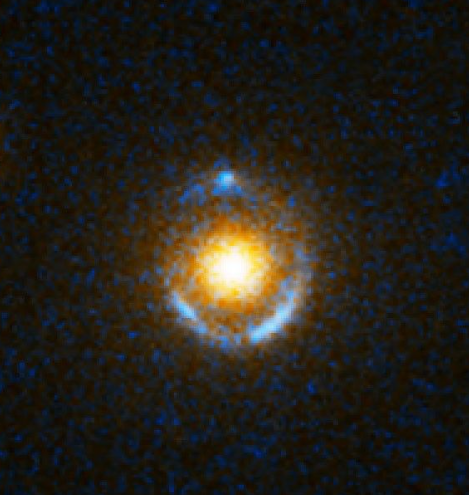
\includegraphics[width=0.5\columnwidth]{Einstein-ring.png}
    \caption{טבעת איינשטיין שצולמה על ידי טלסקופ האבל}
    \label{fig:einstien_ring}
\end{figure}

\textbf{עידוש חלש} הוא המקרה בו תופעות העידוש חלשות מאוד וניתן לזהות את קיום העידוש
והמאפיינים שלו רק בעזרת ניתוח של הרקע כולו.
תופעה זו קוראת לא על ידי עידוש מעצם יחיד אלא על ידי מבני ענק כגון גלקסיות.

\textbf{מיקרו-עידוש} הוא המקרה בו העידוש מתבצע על ידי גוף קטן יחסית, ולא ניתן לראות
את הדמויות השונות באופן אופטי, אך ניתן לראות שינוי בבהירות הגוף שמרמז על מעבר של עצם
מסיבי בין הגוף לבין הצופה.
ההפרדה ניתנת תיאורתית לצפיה, אך כושר ההפרדה של הטלסקופים הקיימים כיום נמוך מכדי
לאפשר זאת.

\textbf{מיקרו-עידוש}
הוא כלי ייחודי לגילוי גופים חשוכים כגון כוכבי ננס חום וכוכבים נייטרוניים,
שאינם פולטים קרינה מספקת לזיהוי ישיר.
בנוסף, הוא מאפשר חילוץ פרמטרים פיזיקליים כגון מסת הגוף המעדש ומרחקו,
דבר שאינו אפשרי בשיטות צפייה רגילות,
ולכן הוא נחשב לאחת השיטות היעילות ביותר לסקר אוכלוסיית גופים אפלים בגלקסיה.

תופעת העידוש הכבידתי נחקרה רבות מאז נחזתה לראשונה על ידי איינשטיין תחת תורת היחסות
הכללית
\cite{wiki:gravlens}, ומדידתה הייתה אחת ההוכחות הראשונות לנכונותה.
ב-1919 אישר ארתור אדינגטון את סטיית קרני האור במדידות ליקוי חמה
\cite{wiki:eddington1919}.
הרעיון שמיקרו-עידוש יכול לשמש ככלי אסטרופיזיקלי לחילוץ מסות עלה בעבודתו של פציינסקי
ב-1986, שהניח את הבסיס לתכניות הסקר המודרניות כגון 
\textenglish{OGLE}.

\subsection*{גדלים תיאורטיים מרכזיים}
\textbf{רדיוס זוויתי}
הוא הזווית הנוצרת בין הצופה לבין גבולות האובייקט הנמדד, ומייצג את הזווית שהאובייקט
תופס בשמיים מנקודת המבט של הצופה, הנמדד בשניות קשת או רדיאנים.
בקירוב זוויות קטנות:
\begin{equation}
    \theta = \frac{R}{D}
\end{equation}
כאשר $R$ הוא רדיוס האובייקט ו-$D$ הוא המרחק לאובייקט.

\textbf{כושר הפרדה},
הנקבע על ידי קריטריון ריילי 
\cite{wiki:angularres}
\mbox{$\theta_{\min} = 1.22\,\lambda/D$},
הוא הרדיוס הזוויתי המינימלי בין שתי נקודות אור כך שיהיה ניתן לראות אותן כנפרדות,
והוא תלוי באורך הגל $\lambda$ של גל האור הנצפה וקוטר הצמצם $D$ של הטלסקופ.

\begin{figure}[H]
    \centering
    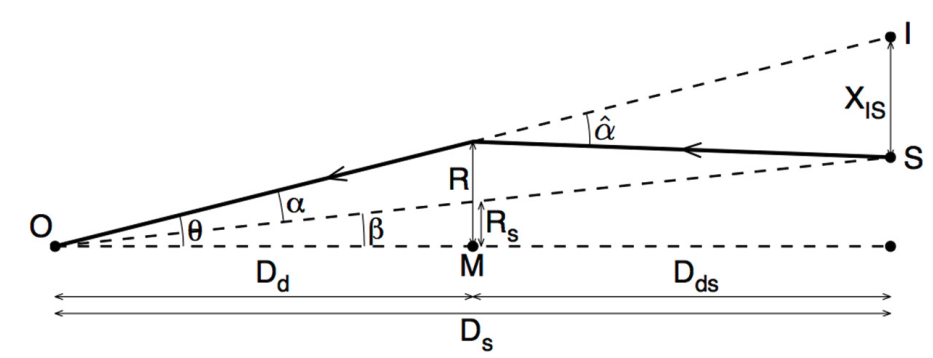
\includegraphics[width=0.7\columnwidth]{lensing_geometry_1.png}
    \caption{גיאומטריית העידוש הכבידתי}
    \label{fig:lensing_geometry_1}
\end{figure}




\textbf{רדיוס איינשטיין}
הוא הרדיוס הזוויתי של הטבעת שנראה בתופעת טבעת איינשטיין.
בנוסף, הוא הרדיוס הזוויתי בו תופעת העידוש הכבידתי מתרחשת באופן משמעותי,
ועקב כך נהוג להשתמש בו כיחידת מידה לזוויות:
\begin{equation}
    \theta_E = \frac{R_E}{D_E}
\end{equation}


רדיוס איינשטין מחושב באמצעות
\begin{align}
    R_E=\sqrt{4\frac{GM}{c^2}D_s\cdot x(x-1)}
    \label{eq:einsteins_radius}
\end{align}

כש-
$G$
ו-
$c$
הם קבוע הכבידה האוניברסלי ומהירות האור בהתאמה.

נוח להגדיר את המשתנה חסר-המימדים $u$, המתאר את היחס בין הזווית האמיתית בין הצופה
למקור האור $\beta$ לבין זווית איינשטיין:
\begin{equation}
    u = \frac{\beta}{\theta_E}
\end{equation}

\textbf{הגדלה} היא תופעה אופיינית לעידוש כבידתי.
השטף המרחבי המוקרן מכוכב כלשהו נשמר, אך בגלל תופעת העידוש קורים שני תהליכים:
הזווית הנצפית של הכוכב גדלה מ-$\beta$ ל-$\theta_\pm$ ובעקבות זאת הכוכב נראה גדול יותר,
ובנוסף, מכיוון שמסת העדשה מעקמת את המרחב-זמן, מוסטים פוטונים מאזורים נרחבים יותר
לכיוון הטלסקופ ואותו אובייקט נראה בהיר יותר.
הגדלת האובייקט המוחלטת מתוארת על ידי $\mu$:
\begin{equation}
    \mu = \frac{F}{F_*} = \frac{u^2+2}{u\sqrt{u^2+4}}
    \label{eq:mu magnification}
\end{equation}
כאשר $F$ ו-$F_*$ הם שטפי הקרינה הנמדדים של כוכב המקור עם ובלי תופעת העידוש, בהתאמה.

נהוג להגדיר את הגודל $u$ בצורה נוספת, הנוחה לעבודה עם מדידות שטף:
\begin{equation}
    u(t) = \sqrt{u_{\min}^2 + t^2}, \qquad t = \frac{T-T_0}{\tau}
\end{equation}
כאשר $u_{\min}$ הוא הערך המינימלי של $u$, המתקבל בזמן $T_0$,
$T$ הוא הזמן הנמדד, ו-$\tau$ הוא הזמן שלוקח למקור לעבור זווית איינשטיין אחת ביחס לעדשה:
\begin{equation}
    \tau = \frac{\theta_E}{\omega}
\end{equation}
כאשר
$\theta_E$
היא זווית איינשטיין ו-
$\omega$
היא התנועה הזוויתית היחסית של המקור
ביחס לעדשה במישור השמיים, תחת הקירוב שהתנועה קווית.

\textbf{מקורות אור נוספים בזמן מדידת אירוע עידוש}

כאשר מבצעים מדידה של אירוע עידוש, עלול להיקלט במדידה מקור אור נוסף שאיננו חלק מאירוע העידוש, ובכך לעוות את התוצאות, טיפול במצב כזה נעזר במספר נוסחאות

נתחיל בלהגדיר גודל הנקרא מקדם הבלנדינג (Blending) 
המוגדר כיחס בין שטף הכוכב $F_s$  לשטף הכולל הנמדד ללא אירוע עידוש $F_{bl}$, המכיל את הכוכב ואת שטף הרקע במדידה
\begin{equation}
    f_{bl} = \frac{F_{source}}{F_{bl}}
    \label{eq:f_bl=F_sorce/F_bl}
\end{equation}
כאשר $f_{bl} = 1$ המשמעות היא שכל השטף הנמדד מגיע מהכוכב המעודש, ולכן ניתוח התצפית לא צריך להתייחס למקורות נוספים, אך כאשר $f_{bl}<1$, המשמעות היא שקיימים מקורות אור נוספים במדידה שיש להתחשב בהם בזמן ניתוח התוצאות

נציין שכאשר פרמטר $f_{bl}<0.5$ המשמעות היא ששטף האור המתקבל מהרקע גדול מהשטף הנקלט מהכוכב, וכתוצאה מכך עקומת האור הנמדדת הולכת ומשטחת ככל שהפרמטר קטן, והופכת את מדידת האירוע והניתוח שלו לקשה מאוד ולא מדוייקת עקב רעש רב שנוצר במדידה על ידי התנודות ברקע, והירידה בהשפעת ההגברה של אירוע העידוש על השטף הכולל, עקב כך שהחלק שאליו אחראי הכוכב מהשטף הכולל, קטן יותר.

בזמן אירוע עידוש השטף הנמדד תואם לנוסחה
\begin{equation}
    F(t) = F_{source} \cdot \mu (t) +F_{background}
    \label{eq:F_source* mu + F_background}
\end{equation}


ומנוסחאות
\ref{eq:f_bl=F_sorce/F_bl},
\ref{eq:F_source* mu + F_background}
מתקבלת הנוסחה
\begin{equation}
    I_{obs}(t) = \frac{F(t)}{F_{bl}} = f_{bl}\cdot\mu(t) + (1-f_{bl})
\end{equation}
כך ש$I_{obs}(t)$ היא ההגברה של העוצמה שמודד הטלסקופ כתוצאה מאירוע העידוש ביחס למדידה ללא אירוע העידוש.



\textbf{המרת מגניטודה לשטף}

מדידות אסטרופיזיקליות של בהירות כוכב נמדדות לרוב במונחי מגניטודה, בצורת מדידה זו, משתמשים בפילטר המאפשר למדוד את בהירות אורך גל מסויים, שנבחר כי ידוע שמתקבל מהכוכב, וככה מונעים רעש מדידה שנוצר ממקורות אחרים, עם זאת, לערך המגניטודה עצמו המתקבל מהמדידה משמעות מעטה בלבד, ונקודת האפס היא שרירותית לגמרי, לכן את הערך הנמדד נהוג להמיר לגודל אחר, בניסוי שלנו אנו ממירים את המגניטודה למונחים של שטף קרינה, על ידי שימוש בנוסחה הבאה
\begin{equation}
    F = F_010^{0.4(m_0-m)}
    \label{eq:trans_m_to_I}
\end{equation}
כך ש $F_0$ ו $m_0$ הם קבועים אופייניים למערכת המדידה.

\textbf{ מסת עדשה}

אחד הגדלים המעניינים ביותר שאנו יכולים לחלץ בעזרת ניתוח מדידות השטף המתקבל ממערכת הוא מסת הגוף המעדש, אותה אנו מוצאים על ידי שימוש בפרמטר $\tau$ וערכים אופייניים של המערכת הנמדדת, והם המרחק לעדשה $D_s$, המהירות של העדשה 
המרחק ביננו לבין המקור $D_d$, יחס המרחקים ביננו לבין העדשה לבין המקור x
\begin{equation}
    x = \frac{D_d}{D_s}
\end{equation}
והמסה M מתקבלת לפי הנוסחה הבאה
\begin{align}
    M&= \frac{(vc\tau)^2}{4x(1-x)GD_s} 
    \label{eq:lens_mass}
\end{align}
    


במאמר זה אנו ממדלים אירועי מיקרו-עידוש כבידתי מנתוני
OGLE
, 
ובפרט את אירוע
\mbox{2008-SMC-001}
ואירוע
\mbox{2008-BLG-002}
תוך שימוש במינימיזציית $\chi^2$ בקירובים לינאריים ולא-לינאריים לחילוץ פרמטרים פיזיקליים כגון $\tau$, $u_{\min}$, מסת העדשה ורדיוס איינשטיין.


\section{שיטות}
\subsection{חלק א'
- 
חישוב
$T_0$
על ידי מינימיזציית 
$\chi^2$ 
עבור מקדמים לינאריים
באירוע 
SMC-001
עם
$f_{bl}=1$
}

אירוע
2008-SMC-001
אינו פרבולי בכל תחום הזמן, ולכן מידלנו אותו רק באזור שיא האירוע, שם הקירוב הפרבולי תקף.
תחילה פיתחנו כלי שמתאים פרבולה לנתונים, תוך שימוש 
באלגוריתם
\textenglish{Barlow}
למינימיזציית
$\chi^2$
\cite{barlowbook}.
לצורך הבדיקה, הופעל הכלי על נתוני דמה בצורת פרבולה עם רעש גאוסי, שנוצרו במטלב.

מקדמי הפרבולה נמצאו על ידי:
\begin{equation}
    \hat{\mathbf{a}} = \left(\tilde{\mathbf{C}}\mathbf{V}^{-1}\mathbf{C}\right)^{-1}
    \tilde{\mathbf{C}}\mathbf{V}^{-1}\mathbf{y}
\end{equation}
והשונות של המקדמים על ידי:
\begin{equation}
    V(\hat{\mathbf{a}}) = \left(\tilde{\mathbf{C}}\mathbf{V}^{-1}\mathbf{C}\right)^{-1}
\end{equation}
כאשר $\mathbf{y}$ הוא וקטור המדידות, $\mathbf{C}$ היא מטריצת התכנון, ו-$\mathbf{V} = \mathrm{diag}(\Delta y_i^2)$ היא מטריצת השונות.

לאחר שנבדקה ההתאמה בין הפרמטרים המדומים לפרמטרים המשוחזרים ונמצא שהסטייה ביניהם קטנה מסטיית תקן אחת, בוצעה סימולציית מונטה קרלו להערכת ביצועי הכלי בממוצע על פני ריצות מרובות.

לאחר מכן הוחל הכלי על נתוני האמת מ-
OGLE 
לאירוע
2008-SMC-001 
\cite{ogle2008smc001}, 
המסופקים בתצורת מגניטודה,
שהומרו לשטף יחסי באמצעות:
\begin{equation}
    \frac{I(t)}{I_*} = 10^{\,(m_* - m(t))/2.5}
\end{equation}



על מנת לקבוע את תחום ההתאמה האופטימלי, הוספנו ללולאת 
\textenglish{for}
שמחשבת את 
$\chi^2_{\rm red}$:
הלולאה מתחילה בנקודה אחת סביב שיא האירוע ומוסיפה נקודות עד שהיא מכסה את כל סט הנתונים.
בסיום הריצה, מוחזרים מקדמי הפרבולה עבור החלון שנתן את ערך 
$\chi^2_{\rm red}$
הקרוב ביותר ל-1.

מהמודל הפרבולי התקבל 
$T_{\max}$
- הזמן שבו ההגדלה 
$\mu(t)$
מקסימלי.


\subsection{חלק ב'
-
חישוב
$\tau$
,
$u_{\min}$
חילוץ רדיוס איינשטיין ומסת העדשה
באירועים
\mbox{SMC-001},
\mbox{BLG-004},
\mbox{BLG-005},
\mbox{BLG-007},
\mbox{BLG-034},
\mbox{BLG-049}
עם
$f_{bl}=1$
}
\label{sec:part2.2}

בחלק זה בוצעה התאמה למודל העידוש הכבידתי הלא-לינארי עבור אירוע
\mbox{SMC-001}
וחמישה אירועים נוספים;
\mbox{BLG-004},
\mbox{BLG-005},
\mbox{BLG-007},
\mbox{BLG-034},
\mbox{BLG-049}
כולם מ2008
שבהם
$f_{bl}=1$.
עבדנו בצורה דומה לחלק הקודם, 
יצרנו מטריצה דו-מימדית פשוטה 
שמייצגת נתוני דמה,
עליה בנינו פונקציית סריקה שבודקת את המינימום הלוקאלי במטריצה על ידי 
אלגוריתם
"\textenglish{Hill-climbing}"
בגרסת מינימום.

עבור תא נבחר התחלתי כלשהו במטריצה,
הפונקציה סורקת את ארבעת התאים הקרובים ביותר לאותו התא,
בודקת באיזה תא מתוך ארבעת התאים שנבחרו ערך
ה-
$\chi^2$
בו
מינימלי מבינהם,
ובנוסף קטן יותר בערכו מהתא ההתחלתי,
 הפונקציה שומרת בזיכרון שאותו תא שעונה על התנאים האלה הוא מינימלי.
 
 לאחר מכן הפונקציה עושה את אותה הבדיקה שתוארה, כשהתא ההתחלתי הוא התא המינימלי שנמצא בצעד הקודם של הפונקציה
 וחוזר חלילה עד שהפונקציה מוצאת שלא קיים תא מבין ארבעת השכנים הקרובים ביותר לתא הנבחר, שנמוך בערכו מהתא הנבחר, 
 אותו תא מוחזר כפלט הפונקציה כנקודת המינימום של המטריצה.

 בעזרת האלגוריתם הזה הורדנו את הסיבוכיות, מסיבוכיות 
 $O(n^2)$
של סריקה פשוטה שעוברת על כל תא במטריצה,
לסיבוכיות מקסימלית
$O(n)$
שמתקבלת במקרה הקיצון שהתא ההתחלתי והתא המינימלי נמצאים בצדדים המנוגדים של האלכסון במטריצה.
דבר זה אפשר לנו להעלות את רזולוציית הסריקה ל-
500
(כלומר מטריצת
$500\text{x}500$).



כשיצרנו את המטריצה עבור נתוני האמת מ-
\textenglish{OGLE},
יצרנו מטריצה דו מימדית
עבור המשתנים 
$\tau$
ו-
$u_{min}$,
עם רזולוציה של 500,
כל וקטור פרמטרים
נבחר להכיל את טווח הנתונים:
$v_i \in [x_{i,0}-5\delta x_i ,x_{i,0}+5\delta x_i]$
כש
$x_{i,0}$
הוא הערך שחושב 
ב
\textenglish{OGLE}
של המשתנה ה-i
ו-
$\delta x_i$
היא אי-הוודאות במשתנה ה-i
מתוך אותן המדידות ב
\textenglish{OGLE},
זאת מתוך הנחה, שבחישוב שלנו, לא תהייה סטייה של יותר מ5 אי-וודאויות מתוך הערך שחושב ב
\textenglish{OGLE}
והטווח הוא באופן יחסי בטוח לעבודה.

נקודת ההתחלה שנבחרה באלגוריתם שצוין לעיל,
היא נקודה בסביבת נקודת המינימום כפי שצוינה במאגר 
\textenglish{OGLE},
ולא נקודה רנדומלית מפאת חיסכון בזמן ריצה.

לאחר
הפעלת האלגוריתם
ומציאת 
$\tau_0$,
$u_{min_0}$
ו-
$\chi^2(u_{min_0},\tau_0)=\chi^2_0$
,שהם הערכים המינימליים שהתקבלו באלגוריתם החיפוש שהוגדר קודם לכן,
בדקנו את ערכי השגיאה שהתקבלו.
כשחיפשנו את ערך השגיאה ב-
$\tau$,
קיבענו את ערך 
$u_{min}$
ל-
$u_{min_0}$.
בדקנו עבור איזה ערך
$\Delta\tau$
מתקבל

\mbox{$\chi^2(u_{min_0},\tau_0 \pm \Delta\tau)=\chi^2_0 +1 $}
שמהווה סטיית תקן
אחת.
מכיוון שאנו עובדים עם ערכים בדידים ולא רציפים,
הגדרנו פרמטר 
$\text{gap}=0.05$
וחיפשנו למעשה את 
$\Delta\tau$
המקיים

\begin{equation}
    \chi^2(u_{min_0},\tau_0 \pm \Delta\tau)-(\chi^2_0 +1)  < \text{gap}
\end{equation}

הפרמטר 
\textenglish{gap}
מאפשר סטייה של 
$0.05$
במציאת הערך 
$\Delta\tau$.

בחלקים מתקדמים יותר של המחקר, עברנו לעבוד עם טנזורי 
$\chi^2$
עם שלושה וארבעה פרמטרים, מה שהגדיל את זמן הריצה 
ואילץ אותנו להוריד את רזולוציית הסריקה ל-
100 
ו-
40 בהתאם.
מה שגרר ששני הגורמים בצד שמאל של אי השוויון, היו באופן 
קבוע גדולים יותר מהפרמטר,
והגדלה של
\textenglish{gap}
משמעה טווח טעות גדול יותר,
ע״מ להימנע מזה, עברנו לשיטת בדיקה שונה:
עבור ערכי
$\Delta \tau$
שונים,
מחושב ההפרש הבא:

\begin{align}
    \chi^2(\tau_0\pm\Delta \tau) - \chi^2_0  \gtrless  1 
\end{align}


ונשמרות שתי נקודות
$(\Delta\tau_i,\chi^2(\Delta\tau_i))$
שהכי קרובות לנק׳ שבה אי השוויון מתהפך.

לאחר מכן משוערך 
$\Delta \tau$
על-ידי אינטרפולציה פשוטה 
\begin{align}
    |\Delta \tau| =  \Delta\tau_1 + \frac{\Delta\tau_2-\Delta\tau_1}{\chi^2(\Delta\tau_2)-\chi^2(\Delta\tau_1)}\cdot(1-\chi^2(\Delta\tau_1))
\end{align}

במדידות מהסוג הזה, מתקבלות שגיאות אסימטריות
ולכן התקבלו שני ערכי שגיאה 
$\Delta \tau ^+, \Delta \tau ^-$
.
עבור 
$u_{min}$
בוצע אנלוגית אותו התהליך עם הצמדה של 
$\tau=\tau_0$.

לאחר מציאת הפרמטרים 
$\tau_0$
ו-
$u_{min_0}$
ושגיאותיהם,
חושבה מסת העדשה באמצעות
(\ref{eq:lens_mass})
כאשר
$v=150 \:\text{km/s}$ 
היא המהירות היחסית של העדשה.

\mbox{2008-SMC-001} 
הוא אירוע שנמצא בענן מגלן הקטן
\mbox{(\textenglish{Small Magellanic Cloud})}
ונמצא במרחק
\mbox{$D_s=(62.44\pm 0.47)\text{kpc}$}
\cite{smc_distance}.
$x$,
הוא המיקום היחסי של העדשה,
בהיעדר מידע על מיקום העדשה נהוג להניח 
$x=0.5$.

שאר האירועים נמצאים בליבת גלקסיית שביל החלב ומרחקם
\mbox{$D_s=(8.178\pm 0.026)\text{kpc}$}
\cite{blg_distance}.
בנוסף חושב רדיוס איינשטיין בעזרת
\ref{eq:einsteins_radius}
ומסת הכוכב המעדש באמצעות
\ref{eq:lens_mass}.
השגיאות האסימטריות על
$\tau$
ו
$u_{min}$
הופצו לשגיאות אסימטריות על 
$M$
ו-
$R_E$.

לבסוף, שורטטה עקומת האור של אירוע
2008-SMC-001
עם המודל התיאורטי המתאים לפרמטרים שנמצאו.


הפרמטרים עם ערכי השגיאה האסימטריים שלהם, אי הוודאות היחסית והשגיאה היחסית מהערכים ב
-
OGLE 
עבור 
$\tau$
ו-
$u_{min}$
הוצגו לאחר כל החישובים.



\subsection{
חלק ג׳
-
חישוב
$\tau$
,
$u_{min}$
ו-
$T_0$
באירועים
\mbox{SMC-001},
\mbox{BLG-006},
\mbox{BLG-053},
\mbox{BLG-009}
ב-
2008
עם
$f_{bl}=1$
}
\label{subsec:2.3}

בחלק זה, כמו בקודם, בוצעה התאמה למודל עידוש כבידתי לא-לינארי,
עבור אירוע
2008-SMC-001,
ושני אירועים נוספים
SMC-001
ו-
BLG-053
,שניהם גם כן מ-2008.
בשלושת האירועים הפרמטר 
$f_{bl}$
שווה ל-1.

עבדנו בצורה דומה לחלק הקודם, אלא שהפעם המטריצה היא טנזור תלת-מימדי, עקב המעבר להתאמה של שלושה פרמטרים חופשיים שונים.
אותו אלגוריתם 
\textenglish{"Hill-climbing"}
הותאם לעבודה במרחב פרמטרים תלת-מימדי,
כאשר בשלב זה הוא סורק שישה שכנים קרובים,
כלומר 2 כיוונים עבור כל מימד פרמטרי, שאר התהליך נשאר זהה לחלק הקודם.

הסיבוכיות בחלק זה גדלה, ולא בגלל האלגוריתם חיפוש, אלא עקב בניית טנזור 
$\chi^2$ עצמו,
שם יש צורך לחשב כל תא בנפרד,
בחלק הקודם כשהסיבוכיות של בניית הטנזור הייתה 
$O(n^2)$
הבעיה לא הורגשה,
אבל כשהסיבוכיות עלתה ל-
$O(n^3)$
(הסיבוכיות עולה לפי 
$n^d$
כש-d
הוא מימד הטנזור)
נאלצנו להוריד את רזולוציית הסריקה ל-
100.

נק׳ התחלת הסריקה ובחירת אורך הווקטורים של כל פרמטר נשארה זהה לחלק הקודם עם
\mbox{$v_i \in [x_{i,0}-5\delta x_i ,x_{i,0}+5\delta x_i]$},
וזאת על מנת להכיל את אותו טווח אי-וודאות מקובל של $5\sigma$
מהערך של 
\textenglish{OGLE}
וכן שזמן הריצה 
יישאר קצר על ידי אותה בחירה של נקודת ההתחלה.

בחישוב ערכי אי הוודאות במדידה השתמשנו באותו אלגוריתם שהוחל בחלק הקודם. 
השינוי היחיד הוא התאמת הפונקציה כך שתקבל ערכים של שלושה משתנים, שניים סטטיים ומקובעים על המינימום שלהם, השלישי דינמי ועבורו מחפשים את
שתי הנקודות הסמוכות ביותר סביב נקודת היפוך אי השוויון
\mbox{$ \chi^2(Q_{1,0},q_{2,0},Q_{3,0}\pm\Delta Q_3) - \chi^2_0  \gtrless  1 $}
כש-
$Q_i$
הוא פרמטר חופשי
ו-
$Q_{i,0}$
הוא ערך אותו הפרמטר שגורר למינימום
ב-
$\chi^2$.
באותה צורה מחושבת השגיאה עם אינטרפולציה זהה
לזו מהחלק הקודם.

עד כאן, לא קיים הבדל בין שלושת האירועים באופן החישוב.
אלא רק בהתאמת החישוב למרחק האובייקט.
אירוע
2008-SMC-001,
נמצא כאמור בענן מגלן הקטן.
והאירועים
\mbox{2008-BLG-008}
 ו-
 \mbox{2008-BLG-053}
נמצאים בליבת גלקסיית שביל החלב 
ומרחקם
\mbox{$D_s=(8.178\pm 0.026)\text{kpc}$}
\cite{blg_distance}.
לבסוף חושבו מסת העדשה ורדיוס איינשטיין באמצעות
משוואות
\ref{eq:lens_mass}
ו-
\ref{eq:einsteins_radius}
בהתאם,
עם מרחקי הגלקסיה המתאימים,
 והפצת שגיאות אסימטריות.


 
\subsection{
חלק ד׳
-
גזירת 
$\tau$,
$u_{min}$
ו-
$f_{bl}$
באירוע
\mbox{2008-BLG-002}
וחישוב מסת ורדיוס אינשטיין של העדשה
}

בשונה מהחלקים הקודמים, נבחר אירוע 
\textenglish{2008-BLG-002}
שבו 
$f_{bl}$, 
אותו פרמטר שקובע האם יש זיהום אור מאובייקט שמימיי אחר שהטלסקופ לא מסוגל להפריד זוויתית, שונה מ-1.
בחרנו באירוע 
\mbox{2008-BLG-002}
,שבו 
$f_{bl}=0.513$
\cite{ogle_general_data}
(ניתן ללא טווח טעות).
אירוע עם פרמטר בלנדיג שקרוב ל-1,
אינו בחירה טובה, באירוע כזה הכוכב הנוסף כמעט ולא משפיע על שטף האור שמגיע באירוע העידוש הכבידתי, ואין בו דיון מיוחד.
מנגד, אירוע עם פרמטר בלנדיג שקרוב ל-0
משמעו שהכוכב השני מזהם את המדידות, כך שלא ניתן להבחין באירוע העידוש כלל.
בחירה בפרמטר בלנדיג של 0.5 היא מאוזנת ומאפשרת לבחון וללמוד אירועים מהסוג הזה.

עבדנו בצורה זהה לחלק הקודם, טנזור כי בריבוע גם כאן נשאר טנזור בשלושה מימדיי פרמטרים עם 
$\tau$
,
$u_{min}$
ו-
$f_{bl}$
כפרמטרים חופשיים.
וקטור פרמטרים שמוגדר כ-
\mbox{$v_i \in [x_{i,0}-10\delta x_i ,x_{i,0}+10\delta x_i]$},
הרזולוציה נשארה זהה ושווה ל-100,
טווח הסריקה שונה ל-
$10\delta x_i$
בכל כיוון.
האלגוריתם כן מצא את המינימום עבור כי בריבוע בתוך טווח של 
$5\delta x_i$,
אבל בחישובי השגיאה נתקלנו בבעיה שטווח הטעות היה גדול מבחלקים הקודמים 
ולא היה ניתן לקיים את המשוואה 
\mbox{$\chi^2(Q_{i,0}\pm\Delta Q_{i}) - \chi^2_0\gtrless 1$}
בטווח הזה.
מעבר לזאת, לא היה שינוי בחישובי השגיאות, וגם כאן בוצעה אינטרפולציה ע״מ להסיק את ערכי אי-הוודאות במדידה.

כמו בכל חלק, חושבו מסת העדשה ורדיוס איינשטיין 
עם 
\ref{eq:lens_mass}
ו-
\ref{eq:einsteins_radius}
בהתאמה ובוצעה הפצת שגיאות אסימטרית.



\subsection{
חלק ה׳
-
גזירת 
$\tau$,
$u_{min}$
,
$f_{bl}$
ו-
$T_0$
\mbox{2008-BLG-002}
וחישוב מסת ורדיוס אינשטיין של העדשה
}
בחלק זה עבדנו על אותו האירוע שבחלק הקודם,
\mbox{\textenglish{2008-BLG-002}},
כאמור עם 
$f_{bl}=0.513$.
בתוספת על החלק הקודם, כאן השארנו ארבעה פרמטרים חופשיים,
$\tau$,
$u_{min}$,
$f_{bl}$
ו-
$T_0$.
התאמנו את הפונקציה שבונה את
$\chi^2$
לחישוב הנוכחי והוספנו לה את האפשרות לקבל מימד פרמטרים נוסף.
אותה התאמה בוצעה לפונקציה שמחפשת את המינימום בטנזור 
$\chi^2$;
הפונקציה מחפשת את התא השכן אליה מבין שמונת התאים שסביבה (2 כיוונים עבור כל פרמטר).
גם כאן, עקב גדילת הסיבוכיות נאלצנו להקטין את רזולוציית הטנזור, הפעם ל-40, וזאת ע״מ להתמודד עם זמן הריצה שגדל לפי 
$O(n^4)$.

חישובי השגיאות בוצעו בצורה זהה לחלקים הקודמים,
 כשבזמן הפעלת הפונקציה שמחפשת את השגיאה עבור פרמטר מסויים, שאר הפרמטרים מקובעים על הערכים שלהם שגוררים כי בריבוע מינימלי.

וכן כמו בחלקים הקודמים, מסת ורדיוס איינשטין חושבו עם
\ref{eq:lens_mass}
ו-
\ref{eq:einsteins_radius}
בהתאמה, ובוצעה הפצת שגיאות אסימטרית.


\subsection{
חלק ו׳
-
השוואת אלגוריתם המינימיזציה שלנו אל מול האלגוריתם של מטלב
בחישובי חלק ה׳
}
\label{sec:part2.6}
חלק זה בוצע באופן אינטרגלי בחלקים הקודמים במהלך בדיקת  האלגוריתם שלנו ובאופן כללי כביקורת על תהליך העבודה.
בתהליך בניית מפת קווי הגובה של כל אירוע ושל כל זוג פרמטרים באותו האירוע, נוסף על הגרף עצמו, סמן בצבע ירוק שמציג את ערך המינימום של
$\chi^2$
שפונקציית
\textenglish{min}
המובנית ב-
\textenglish{matlab}
מצאה,
לצד הערך המינימום שהאלגוריתם שלנו מצא (באדום),
במקרא הגרף הודפסו ערכי המינימום המתאימים,
ראו איור 
\ref{fig:smc001_chi2}.
 \begin{figure}[H]
     \centering
     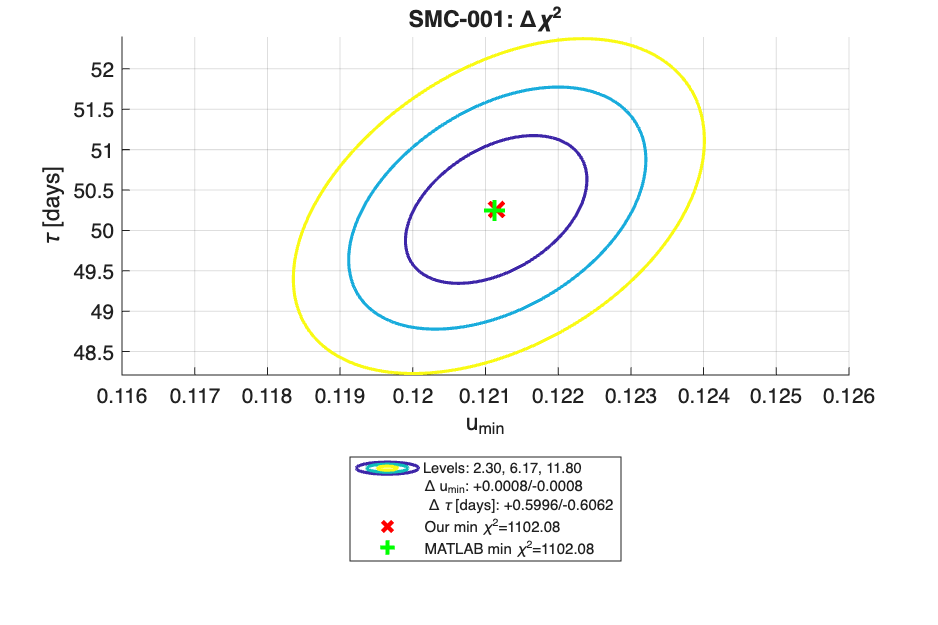
\includegraphics[width=1 \linewidth]{SMC001_chi2.png}
     \caption{גרף קווי גובה,
     אירוע 
     \textenglish{SMC-001}
     מתוך חלק ב׳
     }
     \label{fig:smc001_chi2}
 \end{figure}



יש לציין, לאחר סיום העבודה על האלגוריתם והרצתו על כל חלקי הניסוי 
הגענו למסקנה שניתן היה לשפר את היעליות שלו בכמה מונים.
האלגוריתם כאמור פועל בצורה הבאה, תחילה, נבנה טנזור 
$\chi^2$
באופן מלא, ולאחר מכן האלגוריתם מתחיל את החיפוש שלו בנקודה כלשהי בטנזור ומחפש את המינימום.

הבעיה בגישה הזו היא שהאלגוריתם בונה את הטנזור המלא בגודל 
$\text{res}^d$
כש-$d$
הוא מספר מימדי הטנזור ו\textenglish{res}
הוא מספר האיברים בכל ווקטור בטנזור,
זמן הריצה העיקרי בהרצת האלגוריתם הוא על בניית הטנזור עצמו ולא על מציאת המינימום.

היה ניתן לשלב בין שלבי הפעולה ולהגדיר שהאלגוריתם יפעל בצורה הבאה;
תחילה נבנה טנזור ריק בגדול
$\text{res}^d$
עם הפונקציה 
\textenglish{zeros},
החלק הזה אינו דורש זמן חישוב ומהווה הקצאת זיכרון בלבד,
לאחר מכן, אלגוריתם החיפוש מקבל כקלט את נקודת ההתחלה שלו והוא מחשב את ערכי כי בריבוע של השכנים הסמוכים בלבד,
עבור כל צעד שאלגוריתם החיפוש עושה, יחושבו רק השכנים הסמוכים.
אופן פעולה זה מקטין את סיבוכיות האלגוריתם הכולל (בניית הטנזור + החיפוש) מ-
$O(\text{res}^d)$
ל-
$O(\text{res})$.

כפי שצוין לעיל, ככל שהגדלנו את מרחבי הפרמטרים החופשיים, כך גדל הצורך להקטין את רזולוצית הטנזור, בגישה שתוארה כרגע, היינו נמנעים מכך ומסוגלים אפקטיבית להשאיר את רמת הדיוק בחישוב גבוהה.



\section{תוצאות וניתוח}

מטרת הניסוי היא לנתח מדידות שונות של אירועי מיקרו עידוש, ולחלץ מהן פרמטרים שונים האופייניים לכל אירוע, בתהליך רשמנו תוכנות המאפשרות מציאת מספר ערכים, והם הזמן האופייני לאירוע $\tau$, זמן שיא האירוע 
$T_0$,
המרחק המינימלי בין המקור והעדשה 
$u_{min}$, 
מסת העדשה 
$M$
רדיוס איינשטיין
$R_E$
ופרמטר בלנדינג 
$f_{bl}$
הניתוח נעשה בשלבים, וכלל השוואה בין השגיאות הנעשות על ידי הקירובים השונים.

\subsection{חלק א' - גזירת $T_0$ באירוע \textenglish{SMC-001}}

בחלק זה פיתחנו כלי להתאמה פרבולית של נתונים, המאפשר חילוץ פרמטרי הפרבולה ומיקום השיא שלה. הכלי נבדק תחילה על נתוני דמה סינתטיים. 

לאחר מכן הופעל על נתוני אמת מאתר 
\textenglish{OGLE} 
\cite{ogle_general_data}
עבור אירוע 
\textenglish{2008-SMC-001}.
מהתאמה זו חולץ הזמן 
$T_0$
- רגע השיא של ההגדלה 
$\mu$, 
המתאים למרחק הזוויתי המינימלי בין המקור לעדשה.

\subsubsection*{ניתוח התוצאות }

תחילה הורצה התוכנה על נתוני דמה לבדיקת אמינותה.
נבחרו הפרמטרים
$a = -2,\ b = 2,\ c = 5$,
כך שהשיא של הפרבולה מתקבל בנקודה
$x = 0.5$.
טווח הנתונים שנבחר הוא
$-10 \leq x \leq 10$,
ולכל נקודה נוסף רעש גאוסי אקראי של
$10\%$.

\begin{figure}[H]
    \centering
    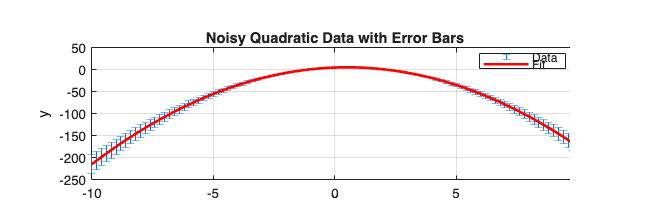
\includegraphics[width=1\linewidth]{part1artifitical.png}
    \caption{התאמה פרבולית לנתוני דמה - בכחול צלבי שגיאה, באדום הפרבולה המותאמת}
    \label{fig:part1_artificial}
\end{figure}
הפרמטרים שהתקבלו:

$a = -2.00 ± 0.02,  b = 2.02 ± 0.02,  c= 5.05 ± 0.05$
הסטייה מהערכים האמיתיים קטנה מסטיית תקן אחת בכל הפרמטרים, המאשרת את אמינות הכלי.

לאחר מכן הופעלה התוכנה על נתוני אמת מאתר
\textenglish{OGLE}.
מכיוון שהנתונים מתקבלים ביחידות מגניטודה, בוצעה המרה לשטף באמצעות נוסחה
\ref{eq:trans_m_to_I}.
הקירוב הפרבולי תקף רק סביב שיא ההגדלה,
גודל חלון הזמנים האופטימלי סביב שיא האירוע נמצא באמצעות לולאה שמחשבת את ערך 
$\chi^2_{red}$
עבור חלונות בגדלים החל מ-
$n=1$
עד לכיסוי האירוע המלא.
חלון הזמנים האופטימלי שנמצא הוא 
n=11,
שהם 22 ימים סביב שיא האירוע
(ראו נספח
\ref{app:chi2_window}).
\begin{figure}[H]
    \centering
    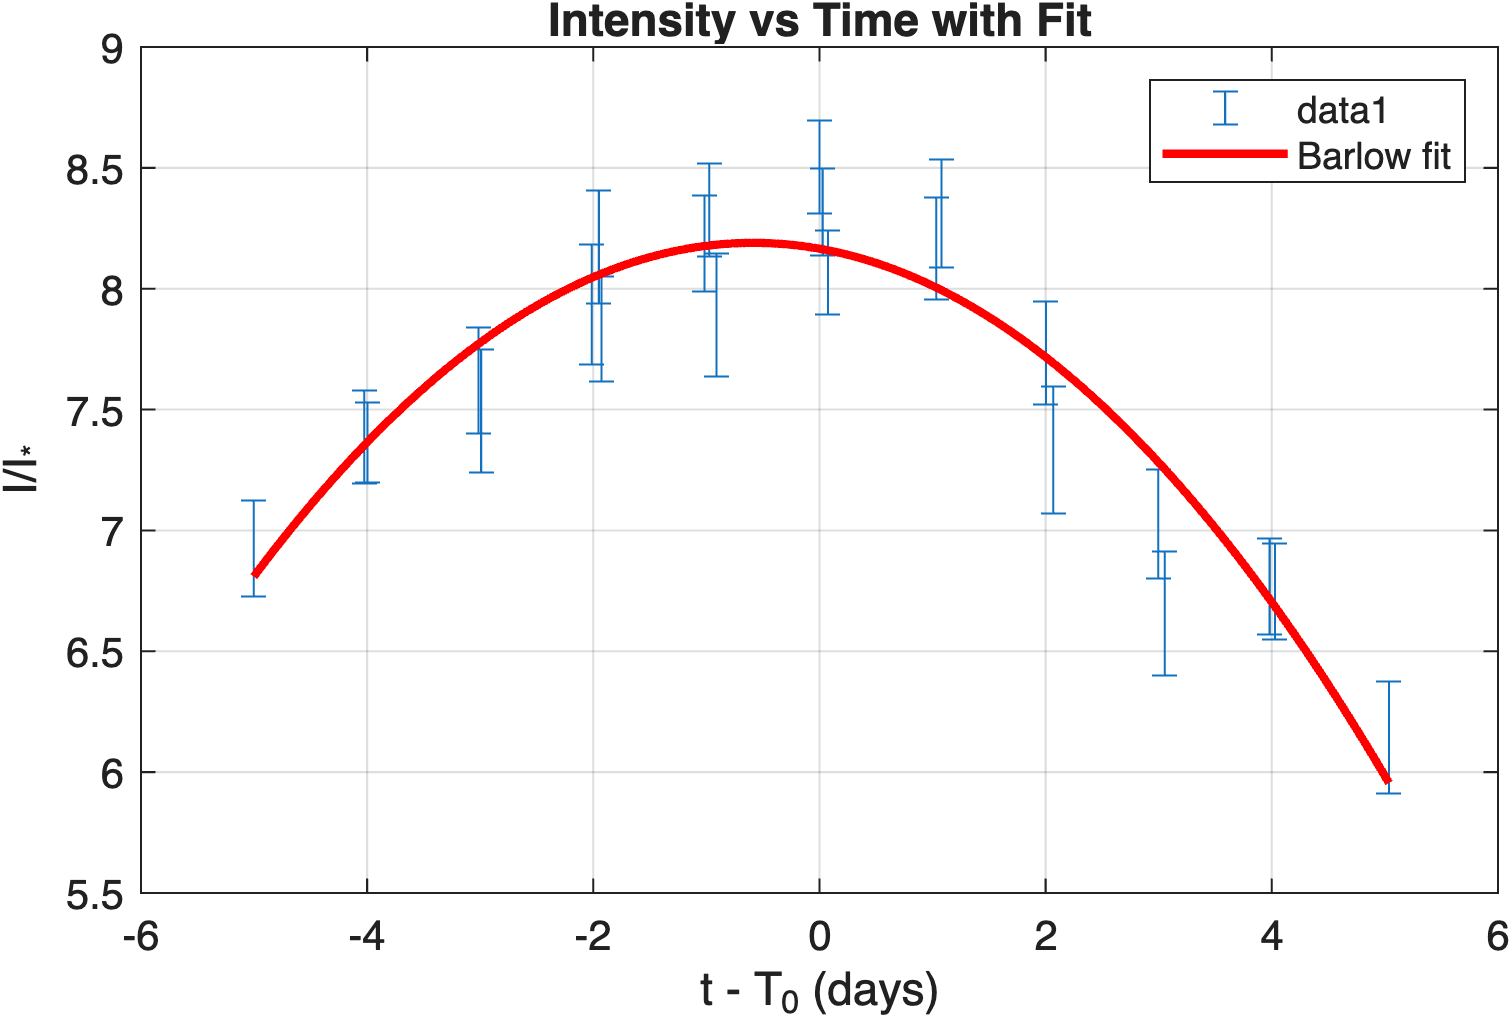
\includegraphics[width=1\linewidth]{part1peak.png}
    \caption{התאמה פרבולית לאזור שיא האירוע
    \textenglish{2008-SMC-001}}
    \label{fig:part1_peak}
\end{figure}

הזמן המתקבל עבור שיא ההגדלה הוא
\noindent\newline
\mbox{$T_0 = 2.45454 \cdot 10^6 \;\text{ [HJD]}$}, 
המהווה שגיאה של
$0.0000035\%$
ביחס לערך של
\textenglish{OGLE}.

\subsection{חלק ב' - גזירת 
$\tau$, 
$u_{\min}$, רדיוס איינשטיין ומסת העדשה באירועי
\textenglish{SMC-001, BLG-004, BLG-005, BLG-007, BLG-034, BLG-049}}
בחלק זה חולצו הפרמטרים
$u_{\min}$
-
היחס הזוויתי המינימלי בין הזווית האמיתית לזווית איינשטיין של האירוע, ו-
$\tau$
-
זמן המעבר של מרחק זוויתי בגודל רדיוס איינשטיין.
הפרמטר
$T_0$
קובע לערך שנמצא ב-
\textenglish{OGLE}
ונשמר קבוע לאורך החישוב.

לאחר מציאת הפרמטרים, חישבנו את מסת העדשה ורדיוס איינשטיין באמצעות
\ref{eq:lens_mass}
ו-
\ref{eq:einsteins_radius}
בהתאמה,
וערכים אופייניים של ענן מגלן הקטן.


\subsubsection*{ניתוח התוצאות}
תחילה נבדקה הפונקציה על נתוני דמה.
הורצה התוכנית על הפונקציה
$Z = a(X-X_0)^2 + b(Y-Y_0)^2$
כאשר
$X_0 = 40,\ Y_0 = -2$.

\begin{figure}[H]
    \centering
    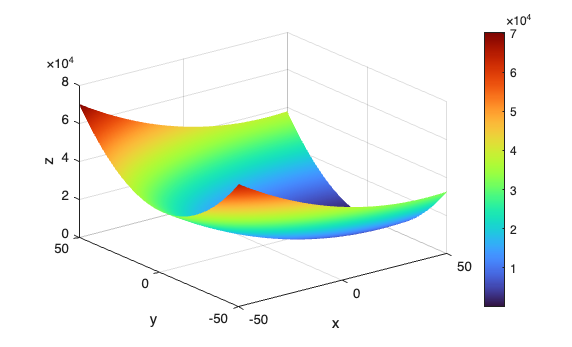
\includegraphics[width=1\linewidth]{part2DammyContour.png}
    \caption{משטח כי בריבוע עבור נתוני דמה פרבוליים}
    \label{fig:part2_dummy}
\end{figure}

המינימום שנמצא הוא
$(X_0, Y_0) = (39.99,\ -1.95195)$,
המהווה שגיאה של
$0.025\%$
עבור
$X$
ו-
$2.25\%$
עבור
$Y$.

מכיוון שהחישוב בדיד, הצירים חולקו ל-1000 יחידות, המייצרים שגיאה של
$0.1$.
הערכים המתקבלים הם
$(X_0, Y_0) = (39.99 \pm 0.1,\ -1.95195 \pm 0.1)$,
ולכן הערכים התיאורטיים נמצאים בטווח השגיאה הצפוי.

לאחר מכן הורצה התוכנית על אירוע
\textenglish{2008-SMC-001}
מאתר
\textenglish{OGLE}.
\begin{figure}[H]
    \centering
    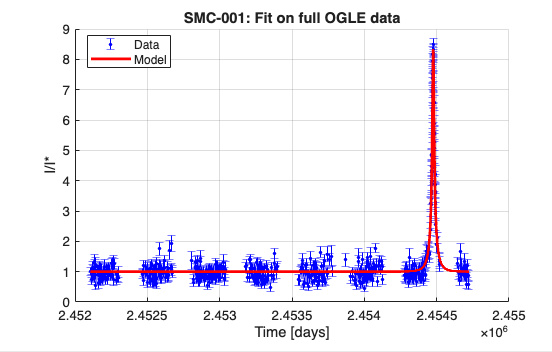
\includegraphics[width=1\linewidth]{001_full.png}
    \caption{עקומת האור של אירוע
    \textenglish{2008-SMC-001}
    עם המודל התיאורטי המותאם}
    \label{fig:001_full}
\end{figure}
הפרמטרים שהתקבלו הם:
\begin{align}
\tau &= 50.2569^{+0.5996}_{-0.6062} \;\text{ [days]} \\
u_{\min} &= 0.1212 \pm 0.0008
\end{align}
המהווים שגיאה של
$1.52\%$
ו-
$0.12\%$
ביחס לערכי
\textenglish{OGLE}
בהתאמה.



ערך כי בריבוע, כלומר טיב ההתאמה של המודל שנמדד עבור אירוע
\mbox{\textenglish{2008-SMC-001}}
הוא
$\chi^2 = 1102.8$
עבור 574 מדידות שונות שבוצעו בנתוני OGLE (דרגות חופש), מתקבל

$\chi^2_{\text{red}} = 1.9267$.


על מנת לבחון את הקורלציה בין הפרמטרים, שורטטה מפת קווי גובה:

\begin{figure}[H]
    \centering
    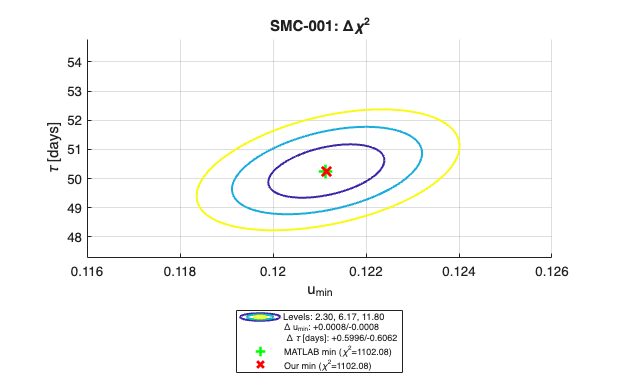
\includegraphics[width=1\linewidth]{part2ContourPlot.png}
    \caption{מפת
    $\Delta\chi^2$
    עבור אירוע
    \textenglish{2008-SMC-001}
    בחלק ב׳}
    \label{fig:part2_contour}
\end{figure}

המינימום שנמצא נמצא בתוך קונטור סטיית תקן אחת, המאשר את אמינות התוצאה.



על אף שויזואלית המינימום נראה במרכז הקונטור, הסטיות המחושבות אינן סימטריות.
עבור
$\tau$,
ההפרש בין השגיאה החיובית לשלילית הוא
$0.006 \; \text{ [days]}$.
אי-סימטריה זו צפויה, עקב התלות הלא-לינארית של המודל ב-
$\tau$
(לפי
\ref{eq:mu magnification}),
בעוד התלות ב-
$u_{\min}$
סימטרית.
בנוסף, המינימום שמצא האלגוריתם שלנו הושווה לזה של פונקציית המינימום המובנית ב-
\textenglish{MATLAB}
- התוצאות זהות, המאשר את אמינות האלגוריתם.

מסת העדשה ורדיוס איינשטיין שחושבו באמצעות נוסחאות
\ref{eq:lens_mass}
ו-
\ref{eq:einsteins_radius}:
\begin{align}
M &= 0.14902^{+0.00372}_{-0.00376}\ M_{\odot} \\
R_E &= 4.3529^{+0.0569}_{-0.0574}\ \text{AU}
\end{align}

התוצאות עבור 5 אירועים נוספים מסוכמות בטבלה
\ref{tab:Mass_and_Radius_part2}

\begin{table}[H]
\centering
\renewcommand{\arraystretch}{1.4} 
\setlength{\tabcolsep}{5pt}
\begin{tabular}{|l|c|c|c|}
\hline
שם האירוע & ($M_\odot$) Mass  & $R_E \;(AU)$  \\ \hline
BLG-004& $1.56895^{+0.00490}_{-0.00489}$ & $0.14782^{+0.00080}_{-0.00079}$   \\ \hline
BLG-005&
$1.51992^{+0.00395}_{-0.00396}$ & $0.13873^{+0.00057}_{-0.00057}$   \\ \hline
BLG-007 & $2.42226^{+0.02340}_{-0.02362}$& $0.35234^{+0.00672}_{-0.00678}$   \\ \hline
BLG-034 &
$5.32501^{+0.00490}_{-0.00489}$ & $1.70278^{+0.03903}_{-0.03804}$ \\ \hline
BLG-049 &
$1.30895^{+0.07914}_{- 0.07581}$ & $0.10289^{+0.01244}_{-0.01191}$   \\ \hline
\end{tabular}
\caption{מסה ורדיוס איינשטיין עבור 5 אירועים}
\label{tab:Mass_and_Radius_part2}
\end{table}

\subsection{חלק ג' - גזירת $\tau$, $u_{\min}$ ו-$T_0$, רדיוס איינשטיין ומסת העדשה באירועי \textenglish{SMC-001, BLG-006, BLG-053, BLG-009}}

בחלק זה הורחב מרחב הפרמטרים לשלושה פרמטרים חופשיים -
$\tau$,
$u_{\min}$
ו-
$T_0$,
במקום לקבע את
$T_0$
לערך
\textenglish{OGLE}.
שחרור פרמטר זה עשוי לשפר את דיוק הערכים המחולצים, במידה וערך
$T_0$
ב-
\textenglish{OGLE}
אינו מדויק.

\subsubsection*{ניתוח התוצאות}
הפרמטרים שהתקבלו עבור אירוע
\mbox{\textenglish{SMC-001}}:
\begin{align}
\tau &= 50.2354^{+0.0621}_{-0.0609} \;\text{[days]} \\
u_{\min} &= 0.12115^{+0.00081}_{-0.00083} \\
T_0 &= 2.45447 \cdot 10^6  \;\text{[HJD]}
\end{align}
$T_0$
מצוין ללא שגיאה כיוון שערך השגיאה היחסית שהתקבל
הוא כ-
$\pm 4.074 \cdot 10^{-8}$.



להלן עקומת האור של האירוע עם המודל התאורטי המותאם לשלושה פרמטרים חופשיים:
\begin{figure}[H]
    \centering
    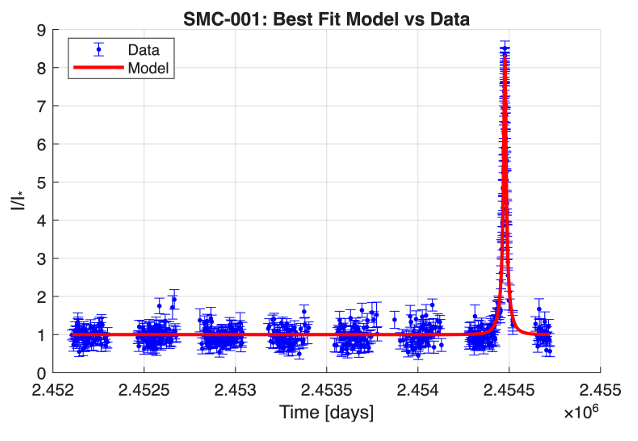
\includegraphics[width=1\linewidth]{Part3Full.png}
    \caption{עקומת האור של אירוע
    \textenglish{SMC-001}
    עם המודל התאורטי - שלושה פרמטרים חופשיים}
    \label{fig:part3_full}
\end{figure}
הטלת
$\Delta\chi^2$
על המישורים השונים מאפשרת בחינת הקורלציה בין הפרמטרים:

\begin{figure}[H]
    \centering
    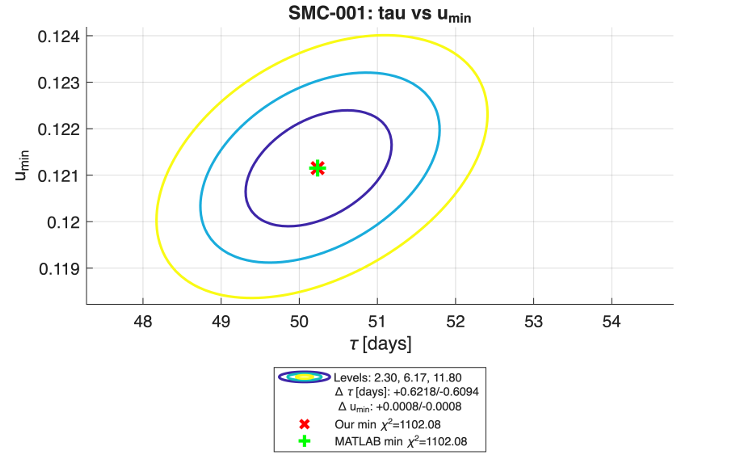
\includegraphics[width=1\linewidth]{contourTau_u.png}
    \caption{מפת
    $\Delta\chi^2$
    במישור
    $\tau$-$u_{\min}$}
    \label{fig:part3_contour_tau_u}
\end{figure}
\begin{figure}[H]
    \centering
    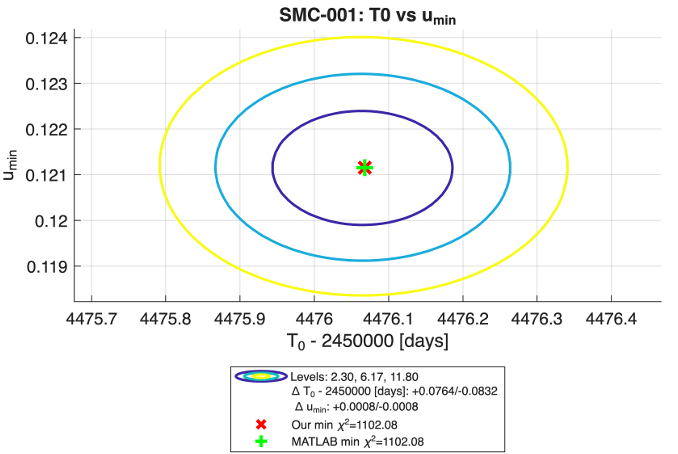
\includegraphics[width=1\linewidth]{cuontourT_u.png}
    \caption{מפת
    $\Delta\chi^2$
    במישור
    $T_0$-$u_{\min}$}
    \label{app:part3_contour_T_u}
    \label{fig:part3_contour_T_u}
\end{figure}
\begin{figure}[H]
    \centering
    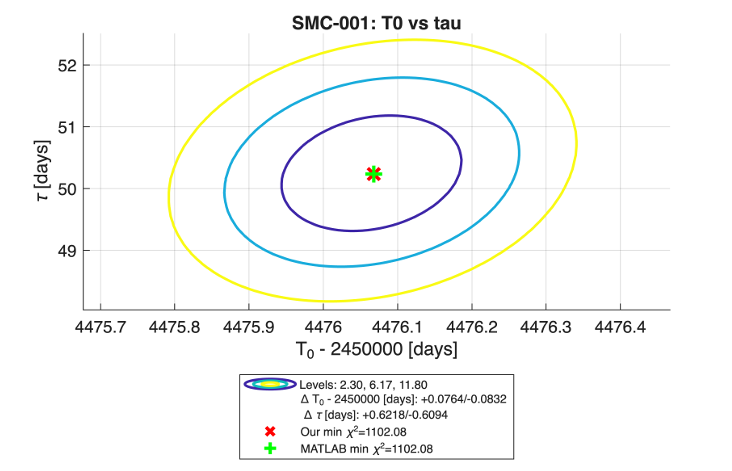
\includegraphics[width=1\linewidth]{contourT_Tau.png}
    \caption{מפת
    $\Delta\chi^2$
    במישור
    $T_0$-$\tau$}
    \label{app:part3contour_T_tau}
    \label{fig:part3contour_T_tau}
\end{figure}




מאיור 
\ref{fig:part3_contour_T_u}
ניתן לראות כי האליפסה אינה נטויה באלכסון אלא מקבילה לצירי הפרמטרים, דבר המעיד על קורלציה חלשה מאוד בין הפרמטר $u_{min}$ לבין זמן שיא האירוע $T_0$.
בנוסף, האליפסה רחבה יחסית לאורך ציר ה-$T_0$, תכונה המצביעה על רגישות נמוכה של המודל לפרמטר זה, כלומר, ניתן לסטות בכ-0.08 ימים (כשעתיים) לכל כיוון מרגע השיא  ועדיין להישאר בתוך תחום של סטיית תקן אחת.

לעומת זאת, קיימת רגישות גבוהה בהרבה לפרמטר
$u_{min}$. 
כפי שנראה מאיורים 
\ref{fig:part3_contour_tau_u}
ו-
\ref{fig:part3_contour_T_u}
, חריגה זעירה של כ-0.0008 לכל כיוון מערך המינימום המיטבי תגרום לתוצאה לצאת אל מחוץ לתחום של סטיית תקן אחת.

מהסתכלות על איורים 
\ref{fig:part3_contour_tau_u}
ו-
\ref{fig:part3contour_T_tau}
ניתן להבחין בא-סימטריה קלה בערכי השגיאה של הפרמטר
$\tau$
\mbox{$(+0.6218 / -0.6094)\:\:[\text{days}]$ },
כפי שצפוי להתקבל עקב התלות הלא-ליניארית של המודל בו.
בנוסף, שיפוע האלכסון הראשי של אליפסת קווי הגובה שאיור
\ref{fig:part3_contour_tau_u} 
נמצא בה מעידה על קורולציה חזקה מאוד בין  
$\tau$
ו- 
$u_{min}$, 
ומאיור
\ref{fig:part3contour_T_tau}
ניתן ללמוד כי קיימת קורולציה מתונה בין $\tau$ ו$T_0$.

יתר על כן, ניתן לראות שההתאמה בין המינימום שמצא האלגוריתם שלנו לחיפוש המינימום מתאים בצורה מדוייקת כמו בחלק ב׳, 
עם זאת,
נציין שעבור אירועים אחרים שניתחנו קיבלנו לפעמים התאמה פחות טובה בין ערכי המינימום שלנו ושל 
\textenglish{Matlab},
הבדל זה נובע מכך שנאלצנו להוריד את רזולוציית הטנזור מ-500 ל-100, מה שהגדיל את ההבדל בערכים בתאים הסמוכים בטנזור.
בנוסף חשוב לציין, האלגוריתם מותאם למטריצה או טנזור עם מינימום גלובלי אחד ואינו מסוגל להתמודד עם ערכי מינימום מרובים, כמו שקיימים לעיתים בטנזורים שחושבו.


מסת העדשה ורדיוס איינשטיין שחושבו באמצעות נוסחאות
\ref{eq:lens_mass}
ו-
\ref{eq:einsteins_radius}:
\begin{align}
M &= 0.14884^{+0.00382}_{-0.00372}\ M_{\odot} \\
R_E &= 4.3510^{+0.0586}_{-0.0576}\ \text{AU}
\end{align}


המהווה שגיאה של
$0.12\%$
מהמסה שהתקבלה בחלק ב'.
ועבור הרדיוס קיימת שגיאה של 
$0.044\%$
מהערך בחלק ב׳.

השגיאות היחסיות ביחס לערכי
\textenglish{OGLE}:
\begin{itemize}[label=$\bullet$]
    \item $T_0$ - שגיאה של $4.07 \cdot 10^{-8}\%$,
    מדויק פי
    $21.5$
    מחלק א'.
    \item $u_{\min}$ - שגיאה של $0.125\%$,
    דומה לתוצאת חלק ב'.
    \item $\tau$ - שגיאה של $1.561\%$,
    דומה לתוצאת חלק ב'.
\end{itemize}

המעבר משניים לשלושה פרמטרים חופשיים לא שיפר משמעותית את דיוק
$\tau$
ו-
$u_{\min}$.
השיפור המשמעותי התקבל בדיוק
$T_0$,
עקב המעבר מקיבוע ערכו לחישובו כפרמטר חופשי.



בנוסף, הרצנו את התוכנית עבור 4 אירועים נוספים:
\begin{table}[H]
\centering

\label{tab:event_parameters_original}
\renewcommand{\arraystretch}{1.4} 

\begin{tabular}{|c|c|c|c|}
\hline
\textbf{אירוע} & \textbf{\begin{tabular}[c]{@{}c@{}}$T_0 \ [\cdot 10^6 \text{ HJD}]$\end{tabular}} & \textbf{\begin{tabular}[c]{@{}c@{}}$\tau$ \\ {[}days{]}\end{tabular}} & \textbf{$u_{min}$} \\ \hline
BLG-006 & $2.45452_{-0.00}^{+0.00}$ & $66.865_{-1.290}^{+1.114}$ & $0.296_{-0.040}^{+0.041}$ \\ \hline
BLG-053 & $2.45453_{-0.00}^{+0.00}$ & $12.173_{-0.971}^{+1.044}$ & $0.287_{-0.012}^{+0.012}$ \\ \hline
BLG-009 & $2.45453_{-0.00}^{+0.00}$ & $28.449_{-0.918}^{+0.941}$ & $0.787_{-0.139}^{+0.138}$ \\ \hline
\end{tabular}
\caption{תוצאות $T_0$, $\tau$, $u_{\min}$ עבור \mbox{BLG-006}, \mbox{BLG-053}, \mbox{BLG-009}}
\end{table}

המהווים שגיאה ביחס לנתוני OGLE של:
\begin{table}[H]
\centering

\label{tab:rel_error_ogle_split}
\begin{tabular}{|c|c|c|c|}
\hline
\textbf{אירוע} & 
\textbf{\begin{tabular}[c]{@{}c@{}}שגיאה ב-$T_0$\\ {[\%]}\end{tabular}} & 
\textbf{\begin{tabular}[c]{@{}c@{}}שגיאה ב-$\tau$\\ {[\%]}\end{tabular}} & 
\textbf{\begin{tabular}[c]{@{}c@{}}שגיאה ב-$u_{min}$\\ {[\%]}\end{tabular}} \\ \hline
BLG-006 & $1.6301 \cdot 10^{-5}$ & $5.0782$ & $0.7432$ \\ \hline
BLG-053 & $1.9646 \cdot 10^{-5}$ & $15.4207$ & $1.4991$ \\ \hline
BLG-009 & $4.4815 \cdot 10^{-6}$ & $1.8853$ & $0.0897$ \\ \hline
\end{tabular}
\caption{שגיאות יחסיות ביחס לערכי OGLE
עבור \mbox{BLG-006}, \mbox{BLG-053}, \mbox{BLG-009}
}
\end{table}


\subsection{חלק ד' - גזירת $\tau$, $u_{\min}$ ו-$f_{bl}$, רדיוס איינשטיין ומסת העדשה באירוע \textenglish{BLG-002}}



בחלק זה ניתחנו אירועים, בהם בזמן המדידה היה נוכח באזור הנמדד, מקור אור נוסף שלא ניתן להפרידו זוויתית, ולכן שטף האור שנפלט ממנו נכלל במדידה כחלק משטף האור הנקלט במדידה, אך ההגדלה עקב אירוע העידוש התקיימה רק עבור הכוכב הנמדד.
בחלק זה קיבענו את הפרמטר $T_0$ על פי המקסימום הנתון מערכי
\textenglish{OGLE},
וחילצנו את הפרמטרים $\tau$, $u_{min}$, $f_{bl}$, והשוונו לערכים שחולצו על ידי 
\textenglish{OGLE},
יחד עם חישוב המסה של העדשה.

\textbf{ניתוח התוצאות}

נציג את גרף ההתאמה הלינארית של המודל, על פי מינימזציה של כי בריבוע עם 3 משתנים חופשיים על האירוע 
\textenglish{BLG-002}.
\begin{figure}[H]
    \centering
    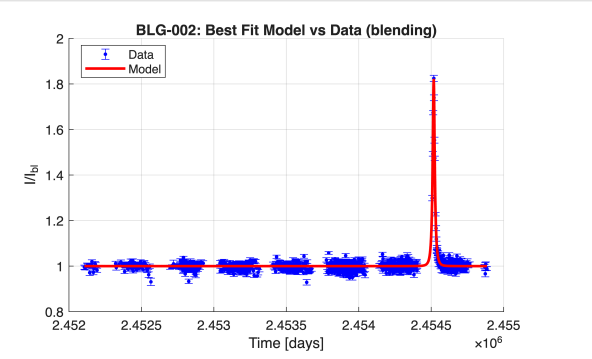
\includegraphics[width=1\linewidth]{Fullpart4.png}
    \caption{עקומת האור של אירוע BLG-002 עם מודל תיאורטי - שלושה פרמטרים חופשיים}

    \label{fig:placeholder}
\end{figure}
ההבדל בניתוח אירועים מסוג זה לבין אירועים בהם מקור האור היחיד הוא הכוכב המעודש, הוא שכעת פרמטר ההגברה $\mu$ מחושב בעזרת נוסחה \ref{eq:mu magnification}.

לאחר התחשבות בתנאי האירועים הללו, כפי שמפורט במבוא התיאורתי ובחלק השיטות
נחלץ את הפרמטרים  $\tau$, $u_{min}$, $f_{bl}$,
הערכים שהתקבלו הם:
\begin{itemize}[label=$\bullet$, noitemsep, topsep=0pt]
\item $\tau = 16.6696^{+ 1.2091}_{-0.9832}\;\text{[days]}$
\item $u_{\min} = 0.4066^{+0.0453}_{- 0.0373}$
\item $f_{bl} = 0.5082^{+0.0038}_{- 0.0080}$
\end{itemize}

המהווים שגיאה ביחס לערכי OGLE של 
0.6519\%
,
1.0567\%
ו-
 0.7299\%
 בהתאמה


כעת נבחן את מפות קווי הגובה עבור הטלת 
$\Delta\chi^2$ 
על שלושת המשתנים, על מנת לבחון את הקורולציה,
בהטלות של $u_{\min}$-$\tau$, $f_{bl}$-$\tau$ ו-$f_{bl}$-$u_{\min}$,
כפי שניתן לראות באיורים.
\ref{fig:part4UminTau},
\ref{fig:part4FblTau},
ו-
\ref{fig:part4FblUmin}
בהתאמה.
 \begin{figure}[H]
     \centering
     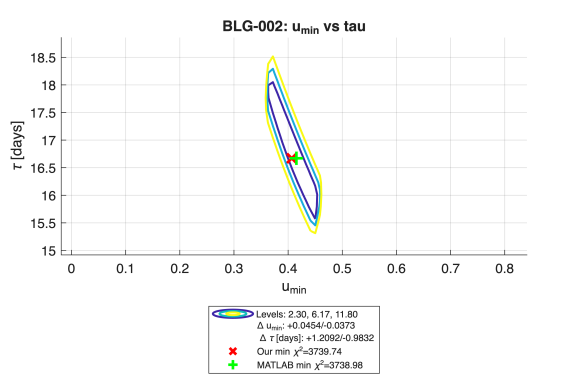
\includegraphics[width=1\linewidth]{part4UminTau.png}
     \caption{מפת $\Delta\chi^2$ במישור $u_{\min}$-$\tau$}
     \label{fig:part4UminTau}
 \end{figure}
\begin{figure}[H]
    \centering
    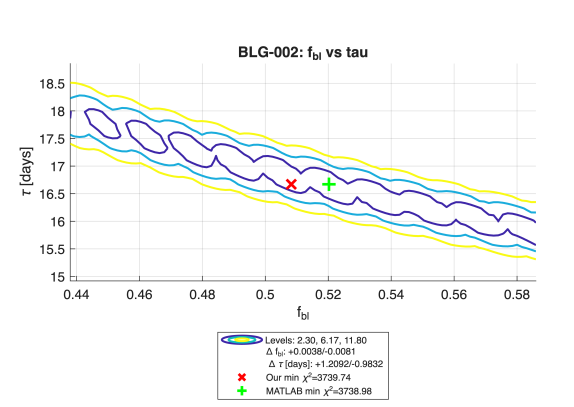
\includegraphics[width=1\linewidth]{Part4FblTau.png}
    \caption{מפת $\Delta\chi^2$ במישור $f_{bl}$-$\tau$}
    \label{fig:part4FblTau}
\end{figure}

\begin{figure}[H]
    \centering
    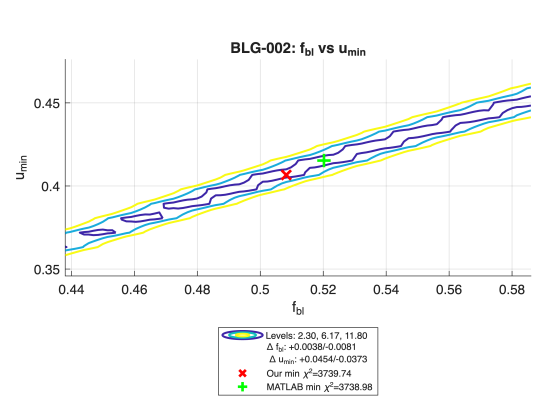
\includegraphics[width=1\linewidth]{Part4FblUmin.png}
    \caption{מפת $\Delta\chi^2$ במישור $f_{bl}$-$u_{\min}$}
    \label{fig:part4FblUmin}
\end{figure}

ניתן לראות כי ערכי המינימום התיאורטיים שמצאנו נמצאים בתוך הקונטור הראשון, המייצג תחום של סטיית תקן אחת, דבר המעיד על אמינות התוצאות ודיוקן הגבוה.

מאיורים \ref{fig:part4FblTau}, \ref{fig:part4FblUmin} ו-\ref{fig:part4UminTau} ניתן להבחין בזווית ובנטייה אלכסונית משמעותית של קווי הגובה, המעידה על קורלציה חזקה מאוד בין שלושת המשתנים.

מבנה האיורים  \ref{fig:part4FblTau} ו \ref{fig:part4FblUmin} נובע מתופעת ניוון, כיוון שקיים מקור אור נוסף,
עם זאת, ניתן לראות בבירור מאיורים \ref{fig:part4FblTau} ו-\ref{fig:part4FblUmin} שטווח ערכי ה-$f_{bl}$ המוגבל על ידי הקונטור הראשון (רמת סטיית תקן אחת) הוא צר מאוד, תכונה זו מצביעה על רגישות גבוהה מאוד של המודל לפרמטר הערבול באזור השיא, כלומר, סטייה קטנה של הניתוח בערך $f_{bl}$ תגרום לסטיה משמעותית מאוד בעקומת המודל התיאורטית ובערך ה-$\chi^2$ וזאת לעומת רגישות מתונה ורחבה בהרבה עבור הפרמטרים $u_{\min}$ ו-$\tau$ המראים אליפסות רחבות ופרושות יותר לאורך ציריהם, נתון שבא לידי ביטוי בערכי השגיאה היחסית הגבוהים של הפרמטרים, 
שהם כ$7.5\%$ בממוצע עבור $\tau$ וכ $10.5\%$ בממוצע עבור$u_{min}$
זאת לעומת שגיאה יחסית של כ$1.1\%$ בממוצע עבור פרמטר $f_{bl}$.






בנוסף נציין שניתן לראות שבהטלות הכוללות את פרמטר $f_{bl}$ קיימת שגיאה משמעותית במציאת המינימום שלנו ביחס למציאת המינימום של MATLAB, הנובעת מכך שרזולוציית המדידה שלנו של 100 נקודות לכל ציר היא מעט נמוכה מכדי למצוא את המינימום בצורה מייטבית, בעיה המחריפה מאוד בחלק זה, בו הקורולציה החזקה בין  הפרמטרים גורמת לאזורי מינימום בעלי מבנה צר ואלכסוני, יחד עם תופעת הניוון הקיצונית במקרה זה,
 שמשמעותה שמספר שילובי פרמטרים שונים יוצרים ערכי $\chi^2$ זהים, ונגרמת עקב כך שבחלק זה ההגברה מושפעת מהפרמטרים $F_{bl}$ ו$u_{min}$, אשר שילובים שונים שלהם יכולים להניב את אותו ערך הגברה, בניגוד לחלק 3 בו ההגברה הייתה תלויה בפרמטר $u_{min}$ בלבד 
 , ולכן נוצרות נקודות מינימום מקומיות רבות שהתוכנית שלנו מתקשה להתמודד איתם בצורה מדוייקת.

 לבסוף חישבנו את מסת העדשה ורדיוס איינשטין באמצעות
 \ref{eq:lens_mass}
ו-
\ref{eq:einsteins_radius}
בהתאמה וקיבלנו את הערכים:
\begin{align}
M &= 0.1251^{+0.0181}_{-0.0147}\ M_{\odot} \\
R_E &= 1.4438^{+0.1048}_{-0.0852}\ \text{AU}
\end{align}
\subsection{חלק ה' - גזירת $\tau$, $u_{\min}$, $f_{bl}$ ו-$T_0$, רדיוס איינשטיין ומסת העדשה באירוע}
חלק זה הוא הרחבה על חלק ד׳ שבו גזרנו את המשתנים 
$\tau$,
$u_{min}$
ו-
$f_{bl}$
באירוע 
\mbox{\textenglish{BLG-002}}
וחושבו בו מסת ורדיוס העדשה,
כעת נשחרר את קיבוע הפרמטר 
$T_0$,
ונחלץ אותו כפרמטר חופשי נוסף.
\subsubsection*{ניתוח תוצאות}
ניתן לראות את המודל שהותאם לנתונים מ
\textenglish{OGLE}
על ידי מינימיזציית כי בריבוע
ואת הנתונים עצמם באיור
\ref{fig:part5_BLG002_fit}.

\begin{figure}[H]
     \centering
     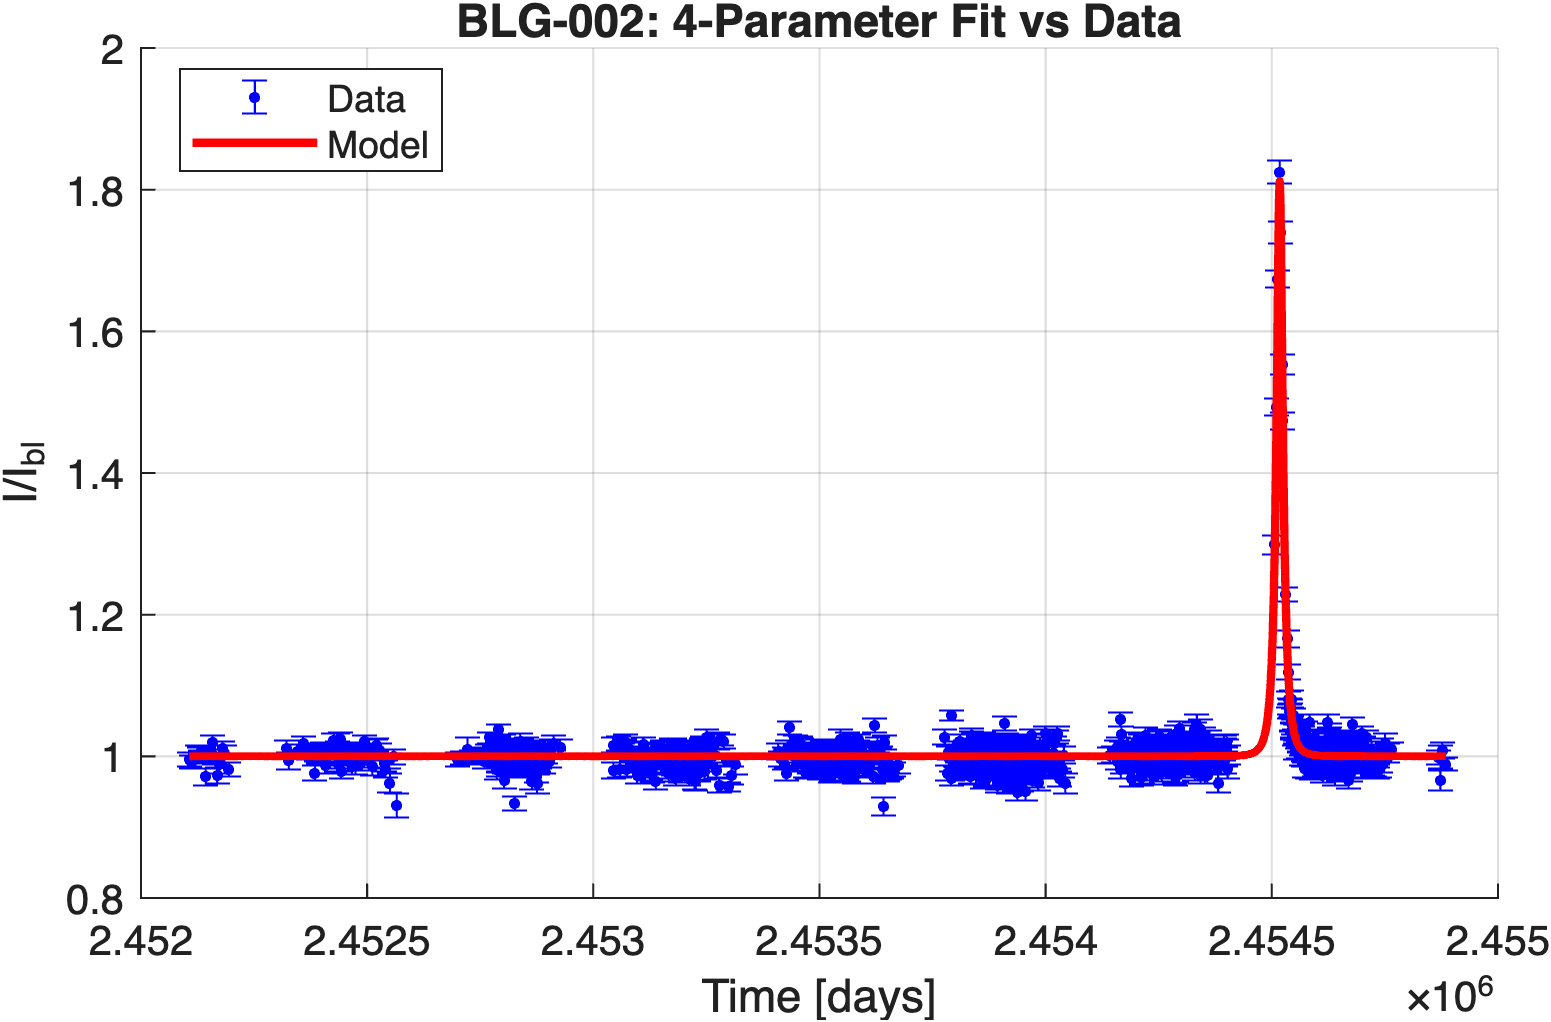
\includegraphics[width=1\linewidth]{Pt5_BLG002_4param_fit.png}
     \caption{עקומת האור של אירוע 
     \mbox{BLG-002}
     עם המודל התאורטי
     -
     ארבעה פרמטרים חופשיים
     }
     \label{fig:part5_BLG002_fit}
 \end{figure}


והפרמטים שהתקבלו במינימיזציית כי בריבוע הם:

\begin{itemize}[label=$\bullet$, noitemsep, topsep=0pt]
    \item $\tau = 16.6401^{+0.0678}_{-0.0560} \;\text{[days]}$
    \item $u_{\min} = 0.4165^{+0.1370}_{-0.2586}$
    \item $f_{bl} = 0.5224^{+0.0064}_{-0.0049}$
    \item $T_0 = 2.4545 \cdot 10^6 \;\text{[HJD]}$
\end{itemize}
השגיאה היחסית בין ערכי 
$\tau$,
$u_{min}$,
$f_{bl}$,
ו-
$T_0$
הם
$3.7185\%$,
$4.7493\%$,
$1.0838\%$
ו-
$3.8335\cdot10^{−5}\%$
בהתאמה,
הגודל של 
$T_0$
נכתב ללא שגיאה כיוון שהשגיאה היחסית היא כ-
$0.000003\%$.

נוסף על כך, ערכי
$\chi^2$
ו-
$\chi^2_{red}$
הם 
$2845.5450$
ו-
$2.1427$
בהתאמה,
כשהשגיאה היחסית בין ערך כי בריבוע המינימלי שחושב על ידנו לבין הערך של מטלב היא:
$0.00065\%$.

ערך 
$\chi^2_{red}$
מחוץ לטווח האידיאלי, אך ניתן להסבירו.
תחילה, נציין שבגלל זמן הריצה של התוכנית, נאלצנו להוריד את רזולוציית הטנזור; בחלק זה הורדנו את הרזולוציה ל-40, ניתן לחשוב שהרזולוציה היא זו שגרמה ל-
$\chi^2_{red}$
לגדול, 
אך מכיוון שההבדל בין ערך 
$\chi^2$
המינימלי שאנחנו ומטלב מצאנו קרובים נורא, אפשר לשלול את הטענה הזו.

המודל שלפיו עבדנו הינו מודל שמניח כוכב נקודתי, עדשה נקודתית, תנועה קווית ו
$f_{bl}$
קבוע, כמובן שבמציאות אף אחת מההנחות האלה לא מתקיימת ועל-כן אי ההתאמה בין המודל לבין האובייקט הנמדד משתקפת בערך 
$\chi^2_{red}$
הגבוה.

בנוסף צריך לקחת בחשבון שהערכת השגיאה אינה אופטימלית, וכנראה גדולה יותר ממה שצוין ב
\textenglish{OGLE}, מה שגם כן תורם לגידול באותו הערך.
 
\vspace{0.5cm}
השגיאה היחסית בין תוצאות חלק ד׳ לחלק ה׳:
\begin{itemize}[label=$\bullet$, noitemsep, topsep=0pt]
    \item $\tau$: $|16.6696 - 16.6401| / 16.6696 = 0.177\%$
    \item $u_{\min}$: $|0.4066 - 0.4165| / 0.4066 = 2.435\%$
    \item $f_{bl}$: $|0.5082 - 0.5224| / 0.5082 = 2.794\%$
\end{itemize}

\vspace{0.5cm}
נוסף על כך, הערכים של 
$\tau$
ו-
$u_{min}$
מחלקים ד׳ וה׳ 
נמצאים בתוך סטיית תקן אחת זה מזה, דבר המעיד על עקביות התוצאות בין החלקים.
באשר ל
$f_{bl}$
ההפרש חורג מסטיית תקן אחת, אך נמצא בתוך טווח השגיאה השלילית
$-0.0080$.

$f_{bl}$ 
רגיש מאוד לתלותיות בין 
$f_{bl}$
ל-
$u_{\min}$.
שחרור 
$T_0$ 
בחלק ה׳ שינה את מרחב הפרמטרים, מה שגרם למינימום 
$\chi^2$ 
להימצא בנקודה שונה במעט במרחב 
$f_{bl}$.

מאיור
\ref{fig:part5_tau_umin}
ניתן לראות קורלציה חזקה בין
$\tau$
ו-
$u_{\min}$,
המתבטאת בנטייה אלכסונית של קווי הגובה.
קורלציה זו צפויה, שכן שני הפרמטרים קובעים יחד את צורת עקומת האור.

מאיור
\ref{fig:part5_umin_fbl}
ניתן לראות את התלות בין
$u_{\min}$
ל-
$f_{bl}$,
המתבטאת בקווי גובה בצורת פס ולא אליפסה סגורה.
תופעה זו נובעת מכך ששילובים שונים של
$u_{\min}$
ו-
$f_{bl}$
יכולים להניב את אותו ערך הגברה, ולכן את אותו ערך
$\chi^2$.

מאיור
\ref{fig:part5_tau_fbl}
ניתן לראות קורלציה בין
$\tau$
ו-
$f_{bl}$,
הנובעת מהתלות שתוארה לעיל - שינוי ב-
$f_{bl}$
מחייב שינוי מפצה ב-
$\tau$
על מנת לשמור על אותו ערך
$\chi^2$.
שאר מפות
$\Delta\chi^2$
מוצגות בנספח
\ref{app:part5_contours}.

\begin{figure}[H]
    \centering
    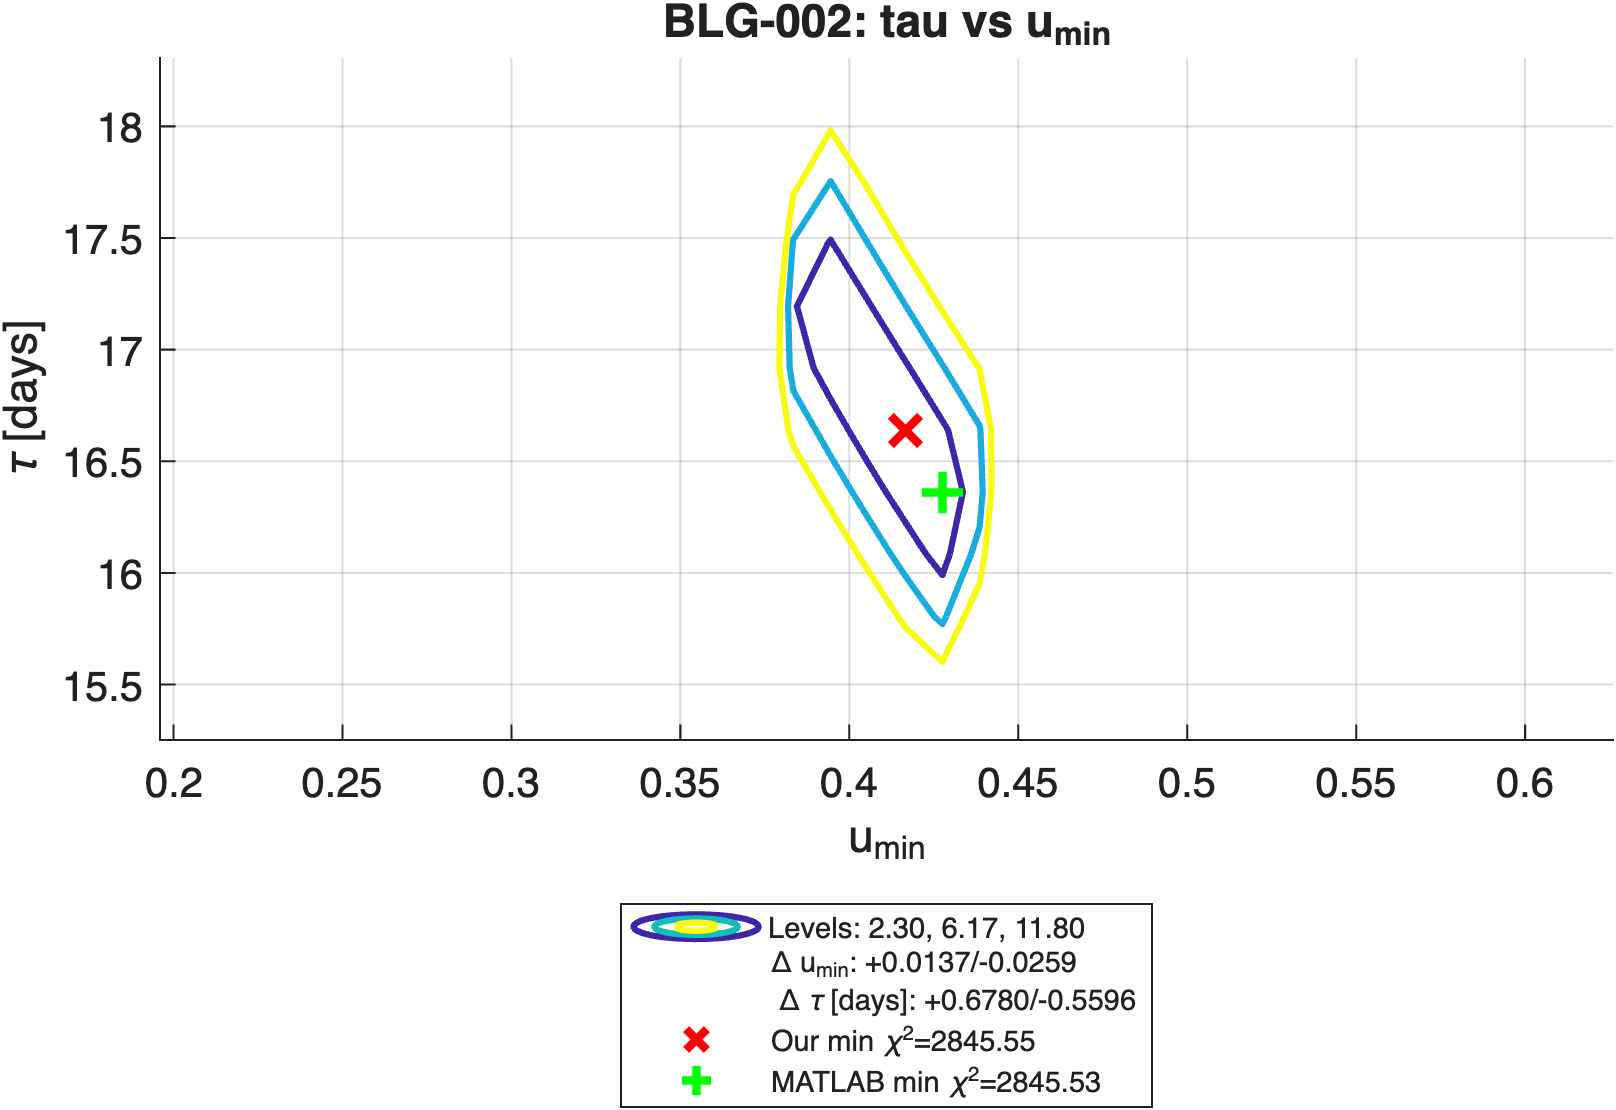
\includegraphics[width=1\linewidth]{Pt5_fig_tau_umin.png}
    \caption{מפת $\Delta\chi^2$ במישור $\tau$-$u_{\min}$}
    \label{fig:part5_tau_umin}
\end{figure}

\begin{figure}[H]
    \centering
    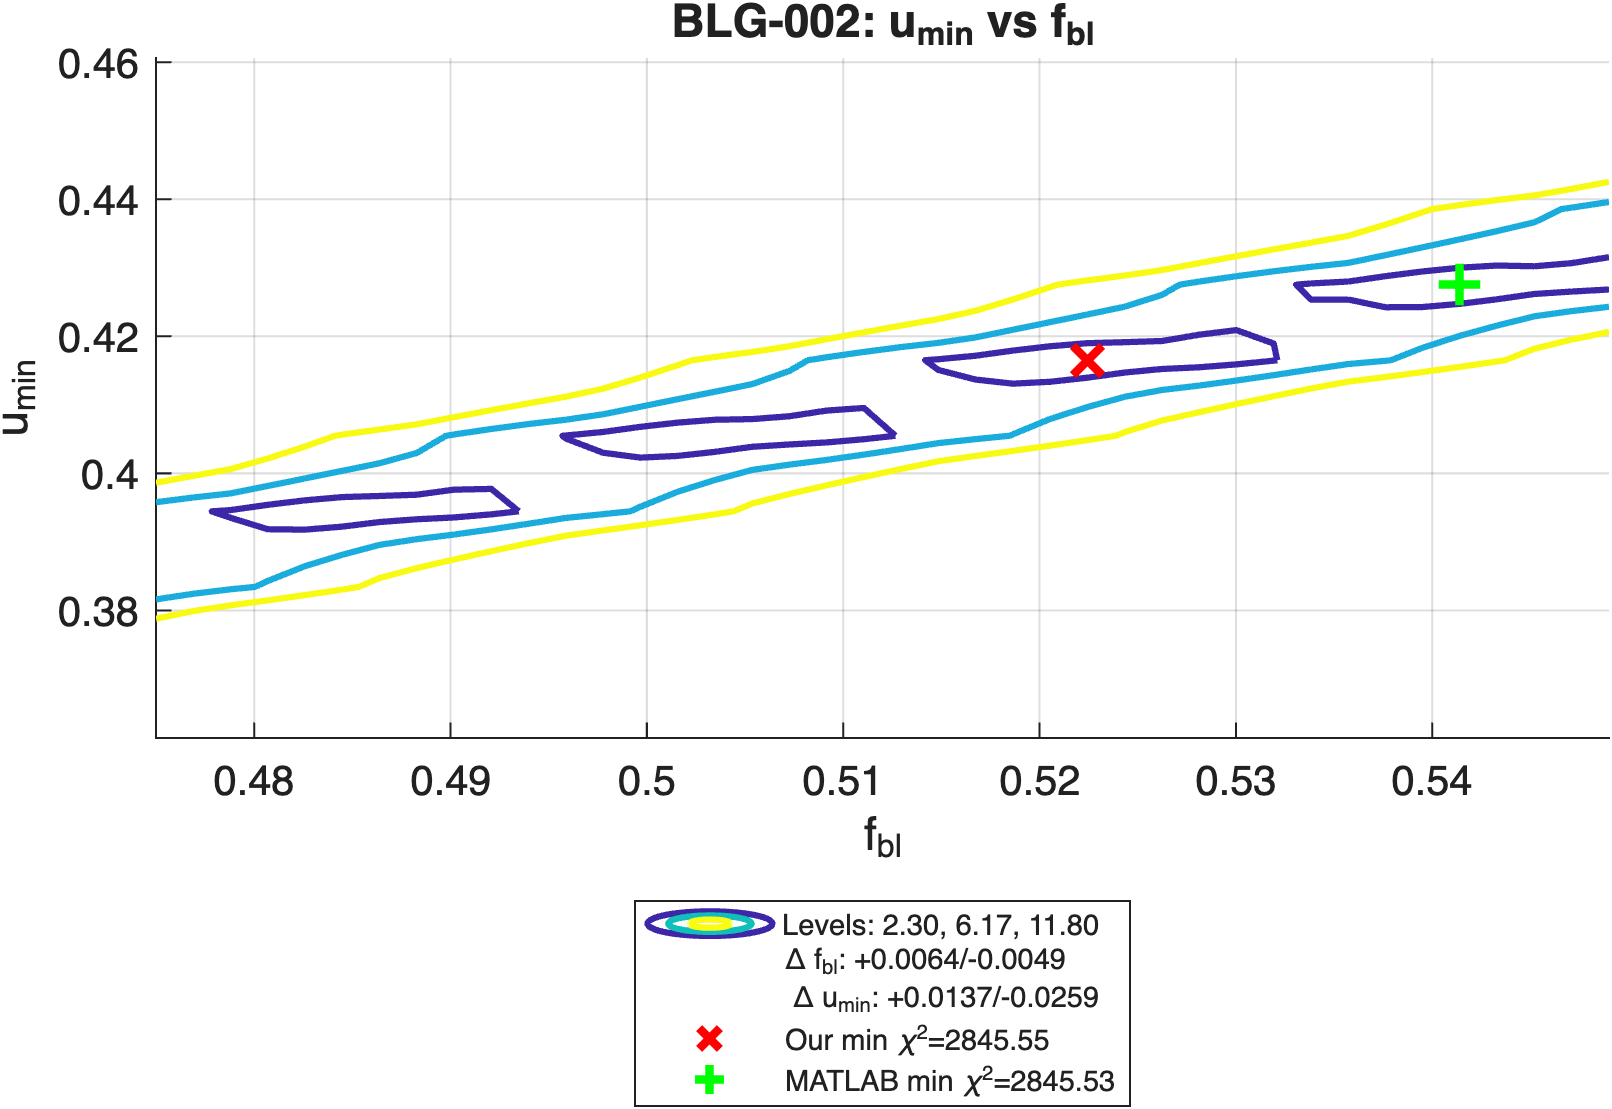
\includegraphics[width=1\linewidth]{Pt5_fig_umin_fbl.png}
    \caption{מפת $\Delta\chi^2$ במישור $u_{\min}$-$f_{bl}$}
    \label{fig:part5_umin_fbl}
\end{figure}

\begin{figure}[H]
    \centering
    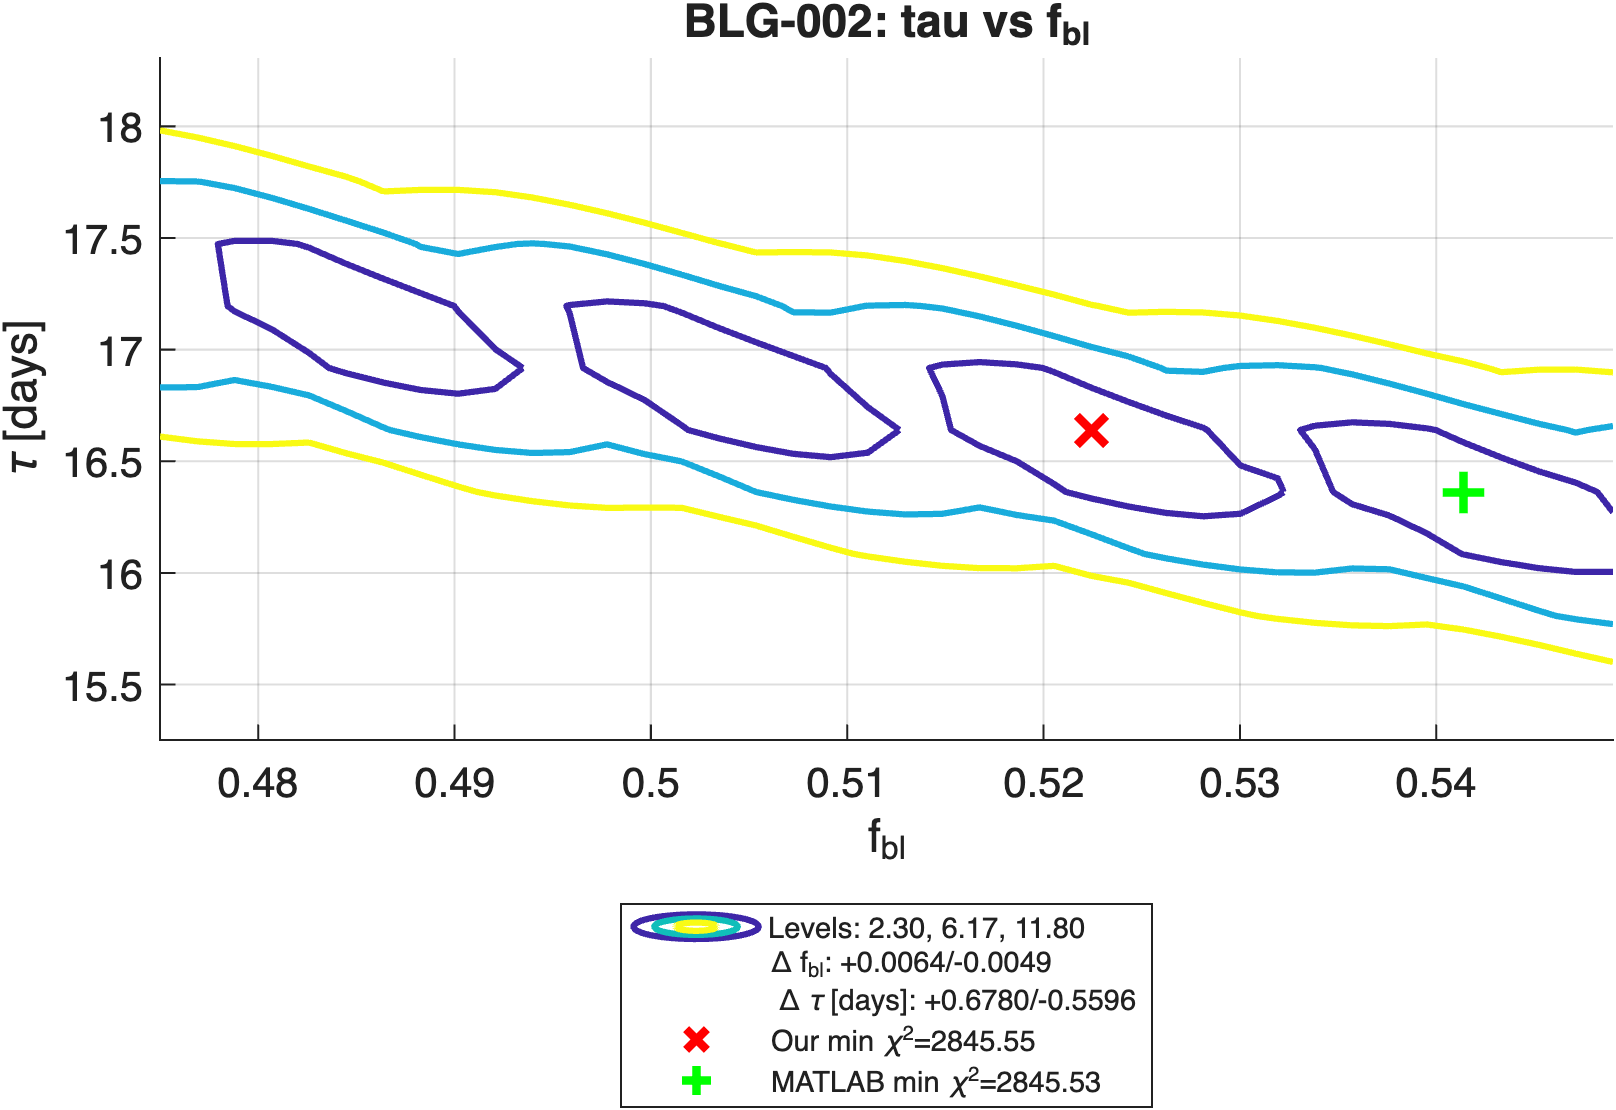
\includegraphics[width=1\linewidth]{Pt5_fig_tau_fbl.png}
    \caption{מפת $\Delta\chi^2$ במישור $\tau$-$f_{bl}$}
    \label{fig:part5_tau_fbl}
\end{figure}


להלן מסת העדשה ורדיוס איינשטיין שחושבו באמצעות נוסחאות
\ref{eq:lens_mass}
ו-
\ref{eq:einsteins_radius}:

\begin{align}
         M &= 0.1247^{+0.1017}_{-0.0840} \cdot 10^{-1}\ M_{\odot}\\
    R_E &= 1.4412^{+0.0588}_{-0.0486}\ \text{AU}
\end{align}




\section{דיון ומסקנות}
בדוח זה ניתחנו אירועי עידוש כבידתי שונים\footnote{
בדיון זה אנו מתמקדים בשני האירועים המרכזיים,
אירוע 
\mbox{\textenglish{2008-SMC-001}}
בחלקים א׳-ג׳
עם 
$f_{bl}=1$,
ואירוע
\mbox{\textenglish{2008-BLG-002}}
בחלקים 
ד׳ ו-ה׳,
עם 
$f_{bl}=0.513$.}
\footnote{\label{fn:footnote_part4}
ניתן למצוא טבלה להשוואת ערכי אי-הוודאות והסטייה מערכי 
\textenglish{OGLE}
לאירועים 
\mbox{\textenglish{2008-SMC-001}}
ו-\mbox{\textenglish{2008-BLG-002}}
בנספח
\ref{app:disscution_compar_methods}.
},
בחלק א׳ עבדנו עם מודל פרבולי של שיא האירוע, בדקנו את התוכנית על נתוני דמה ולאחר מכן על נתוני האירוע מתוך 
\textenglish{OGLE}.
בחלק ב׳ 
השתמשנו במינימיזציית מטריצת 
$\chi^2$
על מנת למצוא את המודל המתאר את האירוע.
בחלק ג׳ השתמשנו באותה שיטה כמו בחלק ב׳ רק ששוחרר פרמטר נוסף והמודל חושב באמצעות מינימיזציית טנזור תלת מימדי של 
$\chi^2$.
לאחר מכן בחלק ד׳
עבדנו על אירוע עם מקדם בלנדינג
$f_{bl}=0.513$,
כאשר נבחרו שלושה פרמטרים חופשיים, והשאר קובעו לערכים מתוך
\textenglish{OGLE},
גם כאן בעזרת מינימיזציית טנזור 
$\chi^2$
נמצא המודל המתאר את האירוע.
בחלק ה׳ בוצע תהליך זהה לחלק ד׳, כאשר נבחרו ארבעה פרמטרים חופשיים.
%\vspace{0.15cm}

\subsection*{חלקים א׳-ג׳,
אירוע 
\mbox{2008-SMC-001}
}
תחילה, בחלק א׳, בנינו תוכנית למציאת זמן שיא האירוע על ידי התאמת מודל פרבולי לחלון זמנים סביב שיא האירוע ומציאת זמן השיא שלו באמצעות גזירת המודל הפרבולי ומציאת נקודת המקסימום של המודל. שיטה זו הניבה מודל מדוייק מאוד, הן לפי השגיאה היחסית הקטנה שהתקבלה והן לפי הסטייה הקטנה מהערכים של 
\textenglish{OGLE}\footref{fn:footnote_part4}.

רמת הדיוק הגבוהה שהתקבלה בדרך הזו נבעה בין היתר, עקב כך שמספר הפרמטרים שעליו רצה התוכנית נמוך מאוד, התוכנית רצה על פונקציה של שני משתנים ולא התייחסה למודל הפיזיקלי המורכב של אירועים מסוג זה, באירועים כאלה כשיש להתאים מספר רב של משתנים, ניתן תחילה למצוא את 
$T_0$
(או כל קבוע שהנתונים שנאספו בניסוי הם פונקציה שלו)
ברמת דיוק גבוהה,
ולאחר מכן להשתמש בו בשלבים מתקדמים יותר בפרמטר מקובע על מנת להבטיח רמת דיוק גבוהה יותר בפרמטרים החופשיים שלא ניתן למצוא בשיטה הזו.
בנוסף, רמת הדיוק הזו נבעה גם עקב כך שבמודל פרבולי כזה ניתן להריץ לולאת 
\textenglish{for}
על חלון הזמן שבו מתייחסים לאירוע כפרבולי,
אותה לולאה שומרת את גודל חלון הזמנים המיטבי שעבורו 
$\chi^2_{red}$
הכי קרוב ל-1,
דבר זה מבטיח, בהתחשב באיכות איסוף הנתונים וקצב הדגימה, שהמודל יהיה מדויק ככל הניתן.

בעזרת שיטה זו מצאנו שזמן שיא האירוע באירוע
\mbox{\textenglish{2008-SMC-001}}
הוא
$T_0 = 2.45448\cdot10^6 \;\text{HJD}$.
עם אי וודאות יחסית ממוצעת של 
$0.0000049\%.$
ושגיאה יחסית מערכי
\textenglish{OGLE}
של-
$0.0000035\%$\footref{fn:footnote_part4}.
\vspace{0.25cm}

\noindent
לאחר מכן, בחלק ב׳, עברנו להשתמש במודל מורכב יותר שמשתמש במינימיזציית מטריצת
$\chi^2$,
כאשר הפרמטרים החופשיים הם 
$u_{min}$
ו-
$\tau$.
המטריצה נבנתה כך שהווקטורים של שני הפרמטרים, מרכזם הוא הערך שנמצא ב-
\textenglish{OGLE},
גודלם הוא 5 סטיות תקן לכל כיוון, והרזולוציה שלהם (כלומר כמה ערכים כל ווקטור מכיל)
היא 500.
בנינו אלגוריתם למציאת מינימום במטריצה שמתבסס על אלגוריתם שנקרא 
"\textenglish{Hill-climbing}"\footnote{
להסבר על האלגוריתם ראו
\nameref{subsec:2.3}.
},
אלגוריתם זה אפשר לנו למצוא את ערך 
$\chi^2$
שעברו התאמת המודל היא אופטימלית.
בעזרת שיטה זו מצאנו שזמן חציית רדיוס איינשטיין 
$\tau$
הוא 
\mbox{$\tau = 50.257^{+0.600}_{-0.606} \text{ days}$}
עם אי וודאות ממוצעת של 
$1.1995\%$,
יחס הזוויות המינימלי
$u_{min}$
שהתקבל הינו
\mbox{$u_{min} = 0.1212 ^{+0.0008}  _{-0.0008}$},
עם אי וודאות יחסית ממוצעת של
$0.679\%$\footref{fn:footnote_part4}.
גם שיטה זו הניבה רמת דיוק גבוהה, עם שגיאה יחסית מערכי 
\textenglish{OGLE}
של כ-
1.59\%
עבור 
$u_{min}$
ו-
0.124\%
עבור 
$\tau$.
בחלק זה התקבל ערך התאמה של
$\chi^2_{red}=1.9267$.
בנוסף עשינו שימוש במפות קווי גובה (מחלק זה ועד חלק ה׳ כולל) שעליהן צוירו ערכי 
$\chi^2$
המינימליים שחושבו על ידי האלגוריתם שלנו ועל ידי האלגוריתם של 
\textenglish{MATLAB}
ששימש כביקורת.
משקל הכוכב המעדש, ורדיוס איינשטיין שלו הם:
\mbox{$M=0.1490^{+0.0037}_{-0.0038}\; M_{\odot}$}
עם אי-ודאות ממוצעת של
\mbox{2.515\%},
ו
\mbox{$R_E = 6.353^{+0.057}_{-0.057}\;\text{AU}$}
עם אי-ודאות ממוצעת של 
$1.312\%$,
בהתאמה.

\vspace{0.25cm}
\noindent
בחלק ג׳, בוצעה מינימיזציה מסוג דומה כמו שצוינה קודם על אותו האירוע 
\mbox{\textenglish{SMC-001}}
כאשר שוחרר פרמטר נוסף כפרמטר חופשי והוא 
$T_0$. 
האלגוריתם שבנינו הותאם לעבודה עם טנזור עם שלושה פרמטרים,
טנזור 
$\chi^2$
עבר גם כן התאמה עקב הגידול בממדים.
מרכז כל ״ווקטור״ בטנזור גם כאן קובע כערך מ-
\textenglish{OGLE}
, גודלם נשאר 5 סטיות תקן לכל כיוון,
אך עקב הגידול בזמן הריצה בבניית טנזור 
$\chi^2$
(בבניית הטנזור מחושב ערך כל תא, כלומר 
$\text{n}^3$
חישובים)
נאלצנו להפחית את רזולוציית הטנזור ל-100, לעומת 500
בחלק הקודם.

זמן החצייה של האירוע
\mbox{\textenglish{SMC-001}}
שהתקבל בשיטה זו הוא
\mbox{$\tau = 50.235^{+0.622}_{-0.609} \;\text{days}$},
עם אי-ודאות ממוצעת של
\mbox{1.226\%}
ושגיאה יחסית של
\mbox{1.561\%}
ביחס לערך
\textenglish{OGLE}.
באופן דומה, יחס הזוויות המינימלי
\mbox{$u_{min} = 0.1212 \pm 0.0008 $}
התקבל עם אי-ודאות ממוצעת של
\mbox{0.678\%}
ושגיאה יחסית של
\mbox{0.125\%}
ביחס ל-
\textenglish{OGLE}.
זמן השיא
\mbox{$T_0 = (2.454476 \pm 0.0000001)\cdot 10^{6}\;\text{HJD}$ }
התקבל בדיוק גבוה במיוחד, עם אי-ודאות ממוצעת של
\mbox{0.0000033\%}
בלבד ושגיאה יחסית של
\mbox{0.0000002\%}
ביחס ל-
\textenglish{OGLE}.
בחלק זה ערך $\chi^2_{red}$
שהתקבל הינו
$\chi^2_{red}=1.9301$.
משקל הכוכב המעדש, ורדיוס איינשטיין שלו הם:
\mbox{$M=0.1489^{+0.0039}_{-0.0038} \;M_{\odot}$}
עם אי-ודאות ממוצעת של
\mbox{2.564\%},
ו-
\mbox{$R_E=4.351^{+0.059}_{-0.058}\;\text{AU}$}
עם אי-ודאות ממוצעת של
\mbox{1.336\%},
בהתאמה.

\vspace{0.25cm}
\noindent
בהשוואה בין שלושת החלקים, ניתן לראות מגמה ברורה:
ככל שמספר הפרמטרים החופשיים במודל גדל,
כך רמת הדיוק (ביחס לערכי
\textenglish{OGLE})
יורדת מעט.
בחלק א׳ התקבלה רמת הדיוק הגבוהה ביותר, עם שגיאה יחסית זניחה של
\mbox{0.0000035\%}
עבור
$T_0$.
בחלק ב׳ ובחלק ג׳, שבהם התאמנו את
$\tau$
ו-
$u_{min}$
(ובחלק ג׳ גם את
$T_0$
כפרמטר חופשי נוסף),
השגיאות היחסיות עלו לסדר גודל של אחוז בודד,
ואי-הוודאויות היחסיות אף הן גדלו בהתאם.

הסיבה המרכזית לפער בין חלק א׳ לשני החלקים האחרים היא ההבדל המהותי בין המודלים:
בחלק א׳ הותאם מודל פרבולי פשוט לחלון זמנים אופטימלי סביב השיא,
ללא צורך להתחשב במודל הפיזיקלי המלא של האירוע.
לעומת זאת, בחלקים ב׳ וג׳ הותאם מודל המבוסס על התיאור הפיזיקלי המלא של תופעת המיקרו עידוש
(פונקציית ההגברה
$\mu(u)$),
מודל זה תלוי במספר פרמטרים חופשיים המתקשרים ביניהם באופן לא ליניארי,
ולכן טעויות בהתאמת פרמטר אחד עלולות להשפיע גם על הפרמטרים האחרים.

בנוסף, בחלק ג׳ נאלצנו להפחית את רזולוציית הטנזור מ-500 (כפי שהיה בחלק ב׳) ל-100,
זאת בשל הגידול המשמעותי בזמן הריצה עם הוספת ממד נוסף לטנזור
$\chi^2$
(מ-
$\text{res}^2$
ל-
$\text{res}^3$
חישובים).
ירידה זו ברזולוציה עלולה להסביר את העלייה הקלה באי-הוודאויות של
$\tau$
ו-
$u_{min}$
בין חלק ב׳ לחלק ג׳
(לדוגמה, אי-הוודאות של
$\tau$
עלתה מ-
\mbox{1.1995\%}
ל-
\mbox{1.226\%}),
שכן רזולוציה נמוכה יותר פוגעת ביכולת לאתר במדויק את נקודת המינימום של
$\chi^2$
ואת נקודות החיתוך המשמשות לחישוב השגיאות האסימטריות.
עם זאת, הפער קטן יחסית, מה שמעיד על כך שהוספת
$T_0$
כפרמטר חופשי לא פגעה באופן משמעותי בדיוק ההתאמה של שאר הפרמטרים,
וכי הרזולוציה שנבחרה (100) הייתה מספקת עבור אירוע זה.

מגמה דומה נראית גם באי-הוודאות של המסה והרדיוס:
אי-הוודאות של המסה עלתה מ-
\mbox{2.515\%}
ל-
\mbox{2.564\%},
ושל הרדיוס מ-
\mbox{1.312\%}
ל-
\mbox{1.336\%},
בהתאמה.
עקביות זו בין כל הפרמטרים התלויים ב-
$\tau$
ו-
$u_{min}$
מחזקת את ההשערה שירידת הרזולוציה היא הגורם המרכזי לפגיעה הקלה בדיוק.



\subsection*{חלקים ד׳-ה׳,
אירוע 
\mbox{2008-BLG-002}
}
חלק ד׳ זהה באופיו לחלק ג׳,
בחנו שם את אירוע
\mbox{2008-BLG-002} 
בלבד,
וכמו בחלק ג׳, השארנו שם שלושה פרמטרים חופשיים.
ההבדל בין חלק ד׳ לחלק ג׳, הוא שבחלק ד׳ נבחר אירוע עם 
מקדם 
\textenglish{blending}
עם 
$f_{bl}=0.513$
ולא,
$f_{bl}=1$
כמו בחלק ג׳.

בחלק זה,
השארנו את הפרמטרים
$\tau$\,
$u_{min}$
ו-
$f_{bl}$
כפרמטרים חופשיים.
גם כאן מרכז ה״ווקטורים״ של כל פרמטר הוא הערך שקיים ב
\textenglish{OGLE},
אך בשונה מהחלקים הקודמים,
גודלו של כל ווקטור הוא 
10
סטיות תקן
(לפי נתוני 
\textenglish{OGLE})
לכל כיוון.

הסיבה לכך היא שבעת חישובי השגיאות האסימטריות, התלותיות בין הפרמטרים הגדילה את האי-וודאות בחלק מהמשתנים,
לעיתים עד כדי כך שלא נמצא  ערך אי וודאות בתוך הטווח המקורי של
5 סטיות תקן לכל כיוון\footnote{
להסבר מפורט יותר על חישובי השגיאה ראו:
\nameref{sec:part2.2}
}.
לאחר מכן, הופעל האלגוריתם, שאפשר לנו למצוא את ערך 
$\chi^2$
שעבורו ההתאמה היא אופטימלית
עם 
$\chi^2_{red}=2.8140$.


הגדלים האופייניים שהתקבלו בחלק זה הינם:
זמן חציית רדיוס איינשטיין
$\tau$
הוא
\mbox{$\tau = 16.670^{+1.209}_{-0.983}\;\text{days}$},
עם אי-ודאות יחסית ממוצעת של
\mbox{6.576\%}
ושגיאה יחסית מערך
\textenglish{OGLE}
של
\mbox{0.652\%}.
יחס הזוויות המינימלי שהתקבל הוא
\mbox{$u_{min} = 0.4067^{+0.0454}_{-0.0373}$},
עם אי-ודאות יחסית ממוצעת של
\mbox{10.169\%}
ושגיאה יחסית מערך
\textenglish{OGLE}
של
\mbox{1.06\%}.
מקדם הבלנדינג שהתקבל הינו
\mbox{$f_{bl} = 0.508^{+0.004}_{-0.008}$},
עם אי-ודאות יחסית ממוצעת של
\mbox{1.170\%}
ושגיאה יחסית מערך
\textenglish{OGLE}
של
\mbox{0.73\%}.

המסה של הכוכב המעדש, ורדיוס איינשטיין שלו, שהתקבלו בחלק זה הם:
\mbox{$M = 0.1252^{+0.0182}_{-0.0148}\;M_{\odot}$},
עם אי-ודאות יחסית ממוצעת של
\mbox{13.156\%},
ו-
\mbox{$R_E = 1.4438^{+0.1048}_{-0.0852}\;\text{AU}$},
עם אי-ודאות יחסית ממוצעת של
\mbox{6.580\%},
בהתאמה.


\vspace{0.25cm}
\noindent
ניתן לראות שרמת הדיוק שהתקבלה בחלק זה נמוכה יותר מזו שהתקבלה בחלקים הקודמים,
כפי שמעיד גם ערך
\mbox{$\chi^2_{red}=2.8140$}
הגבוה יחסית.
הסיבה המרכזית לכך אינה מספר הפרמטרים החופשיים בלבד
(שכן גם בחלק ג׳ הותאמו שלושה פרמטרים חופשיים),
אלא העובדה שבאירוע זה קיים מקדם בלנדינג שונה מ-1.
בלנדינג משמעותי כזה יוצר ,תלותיות בין הפרמטרים
$u_{min}$
ו-
$f_{bl}$,
ניתן לראות זאת במפות קווי הגובה 
(\ref{fig:part4FblUmin})
שבה קווי הגובה מאותו הסדר, מסתדרים בצורה אלכסונית מוארכת, 
מה שמגדיל את הסבירות שערך 
$\chi^2$
המינימלי שהאלגוריתם ימצא, לא יהיה המינימום האמיתי.
עדות נוספת לכך היא הצורך להרחיב את טווח החיפוש ל
10
סטיות תקן לכל כיוון 
(לעומת 5 בחלקים הקודמים)
שכן בטווח המקורי לא נמצאו כלל נקודות החיתוך הדרושות לחישוב השגיאות האסימטריות.
התלותיות הזו בין הפרמטרים היא שמסבירה את ערך 
$\chi^2_{red}$
הגבוה שהתקבל.

בחלק ה׳,
שוחרר גם 
$T_0$
כפרמטר חופשי.
האלגוריתם למציאת המינימום עודכן לקבלת טנזור 4 מימדי,
ושוב בגלל זמן הריצה הגדול (של בניית הטנזור ולא של אלגוריתם החיפוש)
נאלצנו להפחית את רזולוציית הטנזור ל-
40.
באותה דרך כמו קודם בחרנו את מרכזי ה״ווקטורים״ כערכים שהתקבלו ב
\textenglish{OGLE},
גודלם נשאר 5 סטיות תקן (לפי ערכי 
\textenglish{OGLE})
לכל כיוון.

הגדלים האופייניים שהתקבלו בחלק זה הינם:
זמן חציית רדיוס איינשטיין
$\tau$
הוא
\mbox{$\tau = 16.640^{+0.068}_{-0.056}\;\text{days}$},
עם אי-ודאות יחסית ממוצעת של
\mbox{3.718\%}
ושגיאה יחסית מערך
\textenglish{OGLE}
של
\mbox{0.827\%}.
יחס הזוויות המינימלי שהתקבל הוא
\mbox{$u_{min} = 0.4165^{+0.0137}_{-0.0259}$},
עם אי-ודאות יחסית ממוצעת של
\mbox{4.749\%}
ושגיאה יחסית מערך
\textenglish{OGLE}
של
\mbox{1.341\%}.
מקדם הבלנדינג שהתקבל הינו
\mbox{$f_{bl} = 0.5224^{+0.0064}_{-0.0049}$},
עם אי-ודאות יחסית ממוצעת של
\mbox{1.084\%}
ושגיאה יחסית מערך
\textenglish{OGLE}
של
\mbox{2.038\%}.
זמן השיא
\mbox{$T_0 = (2.454517529\pm0.0000001)\cdot10^{6}\;\text{HJD}$}
התקבל בדיוק גבוה במיוחד, עם אי-ודאות יחסית ממוצעת של
\mbox{0.0000038\%}
בלבד ושגיאה יחסית של
\mbox{0.0000004\%}
ביחס ל-
\textenglish{OGLE}.
ההתאמה בחלק זה טובה יותר מההתאמה בחלק ד׳,
שכן התקבל ערך 
$\chi^2_{red}$
נמוך יותר מבחלק הקודם עם 
$\chi^2_{red}= 2.1427$.
המסה של הכוכב המעדש, ורדיוס איינשטיין שלו, שהתקבלו בחלק זה הם:
\mbox{$M = 0.1247^{+0.0102}_{-0.0084}\;M_{\odot}$},
עם אי-ודאות יחסית ממוצעת של
\mbox{7.444\%},
ו-
\mbox{$R_E = 1.4412^{+0.0588}_{-0.0486}\;\text{AU}$},
עם אי-ודאות יחסית ממוצעת של
\mbox{3.876\%},
בהתאמה.



\vspace{0.25cm}
\noindent
בהשוואה בין חלק ד׳ לחלק ה׳, מתקבלת תמונה מעורבת.
מצד אחד, איכות ההתאמה השתפרה, כפי שמעיד ערך
$\chi^2_{red}$
שירד מ-
\mbox{2.8140}
בחלק ד׳
ל-
\mbox{2.1427}
בחלק ה׳,
וכן אי-הוודאויות היחסיות של כל הפרמטרים המשותפים קטנו:
עבור
$\tau$
מ-
\mbox{6.576\%}
ל-
\mbox{3.718\%},
עבור
$u_{min}$
מ-
\mbox{10.169\%}
ל-
\mbox{4.749\%},
ועבור
$f_{bl}$
מ-
\mbox{1.170\%}
ל-
\mbox{1.084\%}.
מצד שני, השגיאה היחסית ביחס לערכי
\textenglish{OGLE}
דווקא גדלה עבור כל שלושת הפרמטרים הללו:
עבור
$\tau$
מ-
\mbox{0.652\%}
ל-
\mbox{0.827\%},
עבור
$u_{min}$
מ-
\mbox{1.06\%}
ל-
\mbox{1.341\%},
ובאופן בולט במיוחד עבור
$f_{bl}$,
שהשגיאה בו כמעט השתלשה
מ-
\mbox{0.73\%}
ל-
\mbox{2.038\%}.
$T_0$
עצמו, שהתווסף כפרמטר חופשי חדש בחלק זה, התקבל בדיוק גבוה במיוחד ביחס ל-
\textenglish{OGLE}.
יש לציין שבין שני החלקים השתנו מספר גורמים בו-זמנית -
מספר הפרמטרים החופשיים (משלושה לארבעה),
רזולוציית הטנזור (מ-100 ל-40),
וטווח החיפוש (מ-10 ל-5 סטיות תקן) -
ולכן קשה לבודד את השפעתו של כל גורם בנפרד על מגמות אלו.
עם זאת, ניתן לשער שרזולוציה גבוהה יותר בחלק ה׳,
כפי שהייתה מתאפשרת עם יישום הגרסה היעילה יותר של האלגוריתם המתוארת בסעיף
\ref{sec:part2.6},
הייתה עשויה לצמצם את הפער מערכי
\textenglish{OGLE}
שנצפה בעיקר בפרמטר
$f_{bl}$.













\newpage
\section*{ביבליוגרפיה}

\begin{LTR}
\printbibliography[heading=none]
\end{LTR}

\appendix
\renewcommand{\thesection}{\alph{section}}
\section{נספחים}
\setcounter{figure}{0}
\renewcommand{\thefigure}{\thesection.\arabic{figure}}
\renewcommand{\figurename}{נספח}

\subsection{התפלגות $b_m$}
\label{app:b_m_sec}
\begin{figure}[H]
    \centering
    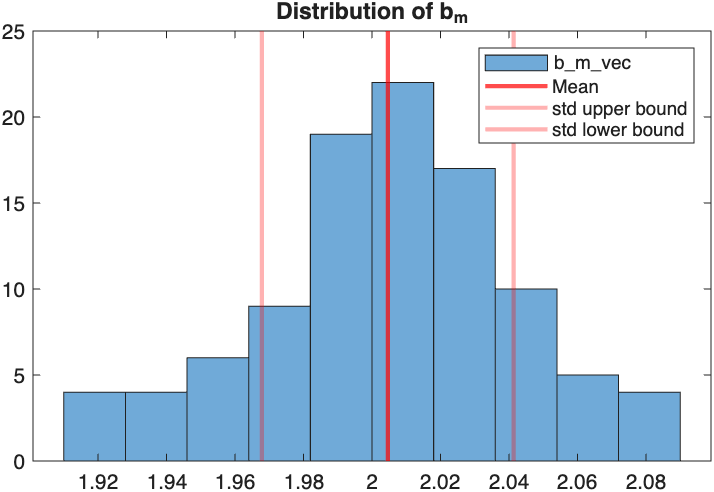
\includegraphics[width=0.5\columnwidth]{b_m.png}
    \caption{היסטוגרמה $b_m$}
    \label{app:b_m}
\end{figure}

\subsection{התפלגות $c_m$}
\label{app:c_m_sec}
\begin{figure}[H]
    \centering
    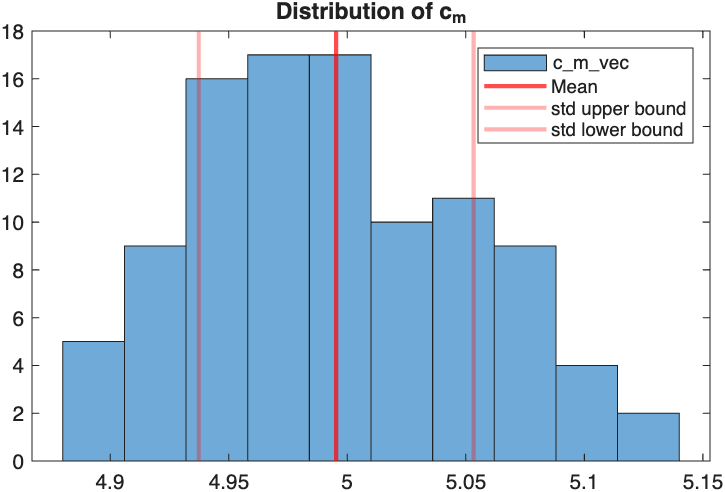
\includegraphics[width=0.5\columnwidth]{c_m.png}
    \caption{היסטוגרמה $c_m$}
    \label{app:c_m}
\end{figure}


\subsection{גרף $\chi^2$ כפונקציה של חלון}
\label{app:chi2_window_sec}
\begin{figure}[H]
    \centering
    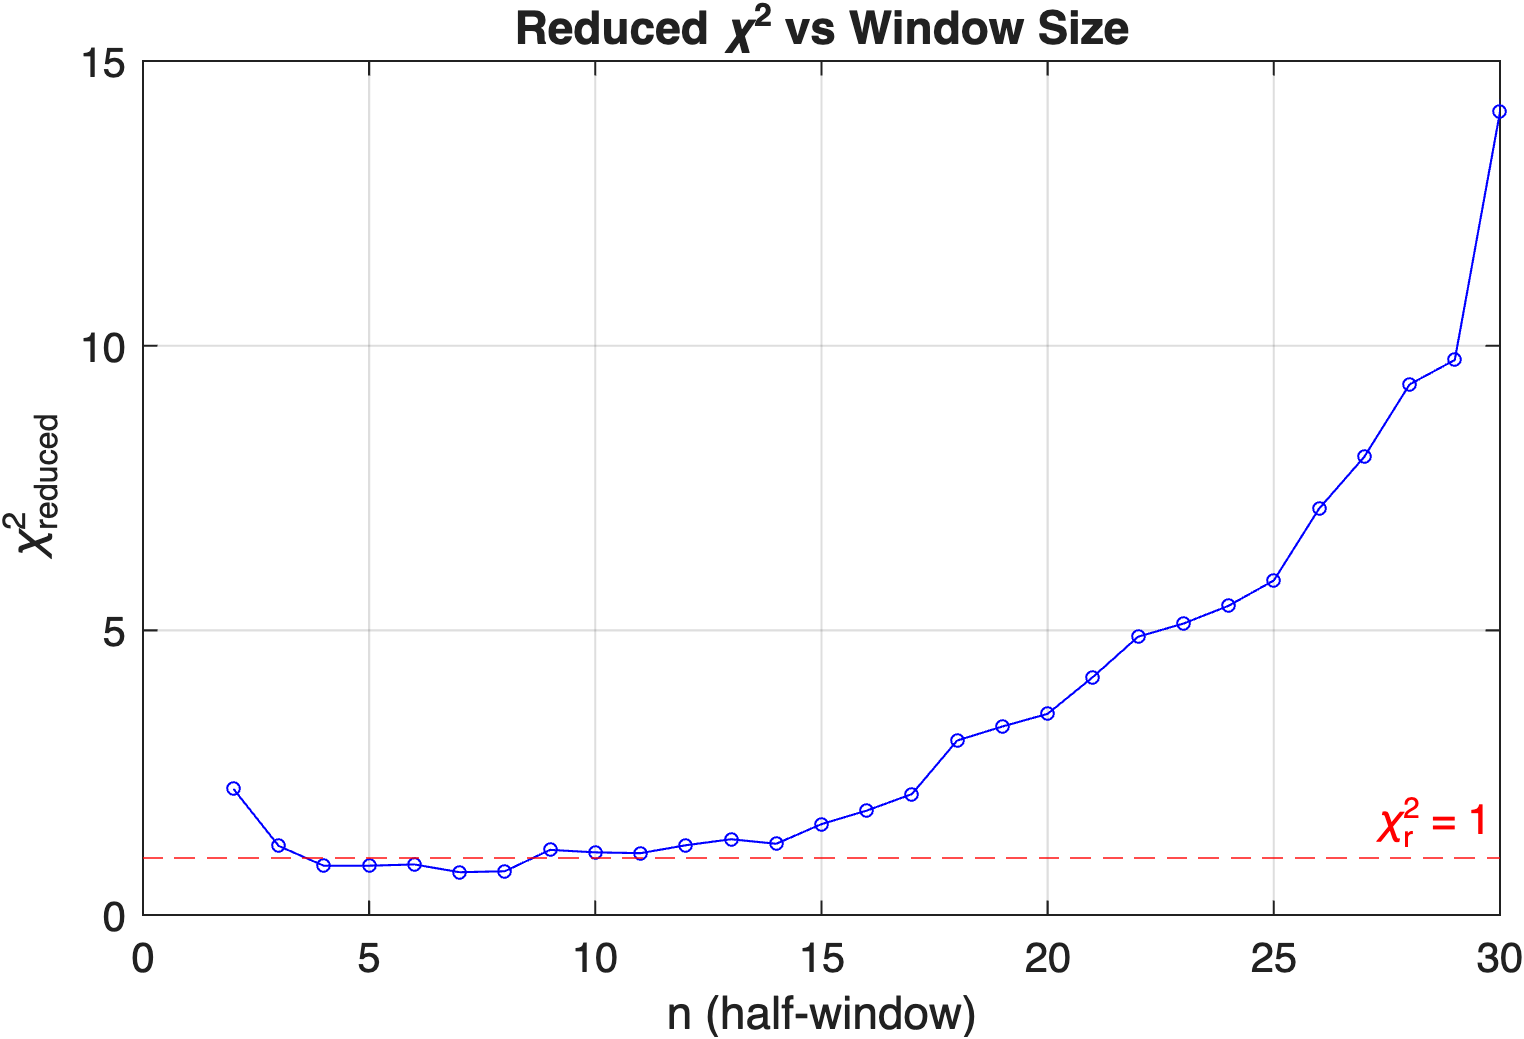
\includegraphics[width=\columnwidth]{chi2_window.png}
    \caption{$\chi^2_{\text{red}}$ כפונקציה של גודל החלון}
    \label{app:chi2_window}
\end{figure}


\subsection{מפות $\Delta\chi^2$ - חלק ה׳}
\label{app:part5_contours}
\begin{figure}[H]
    \centering
    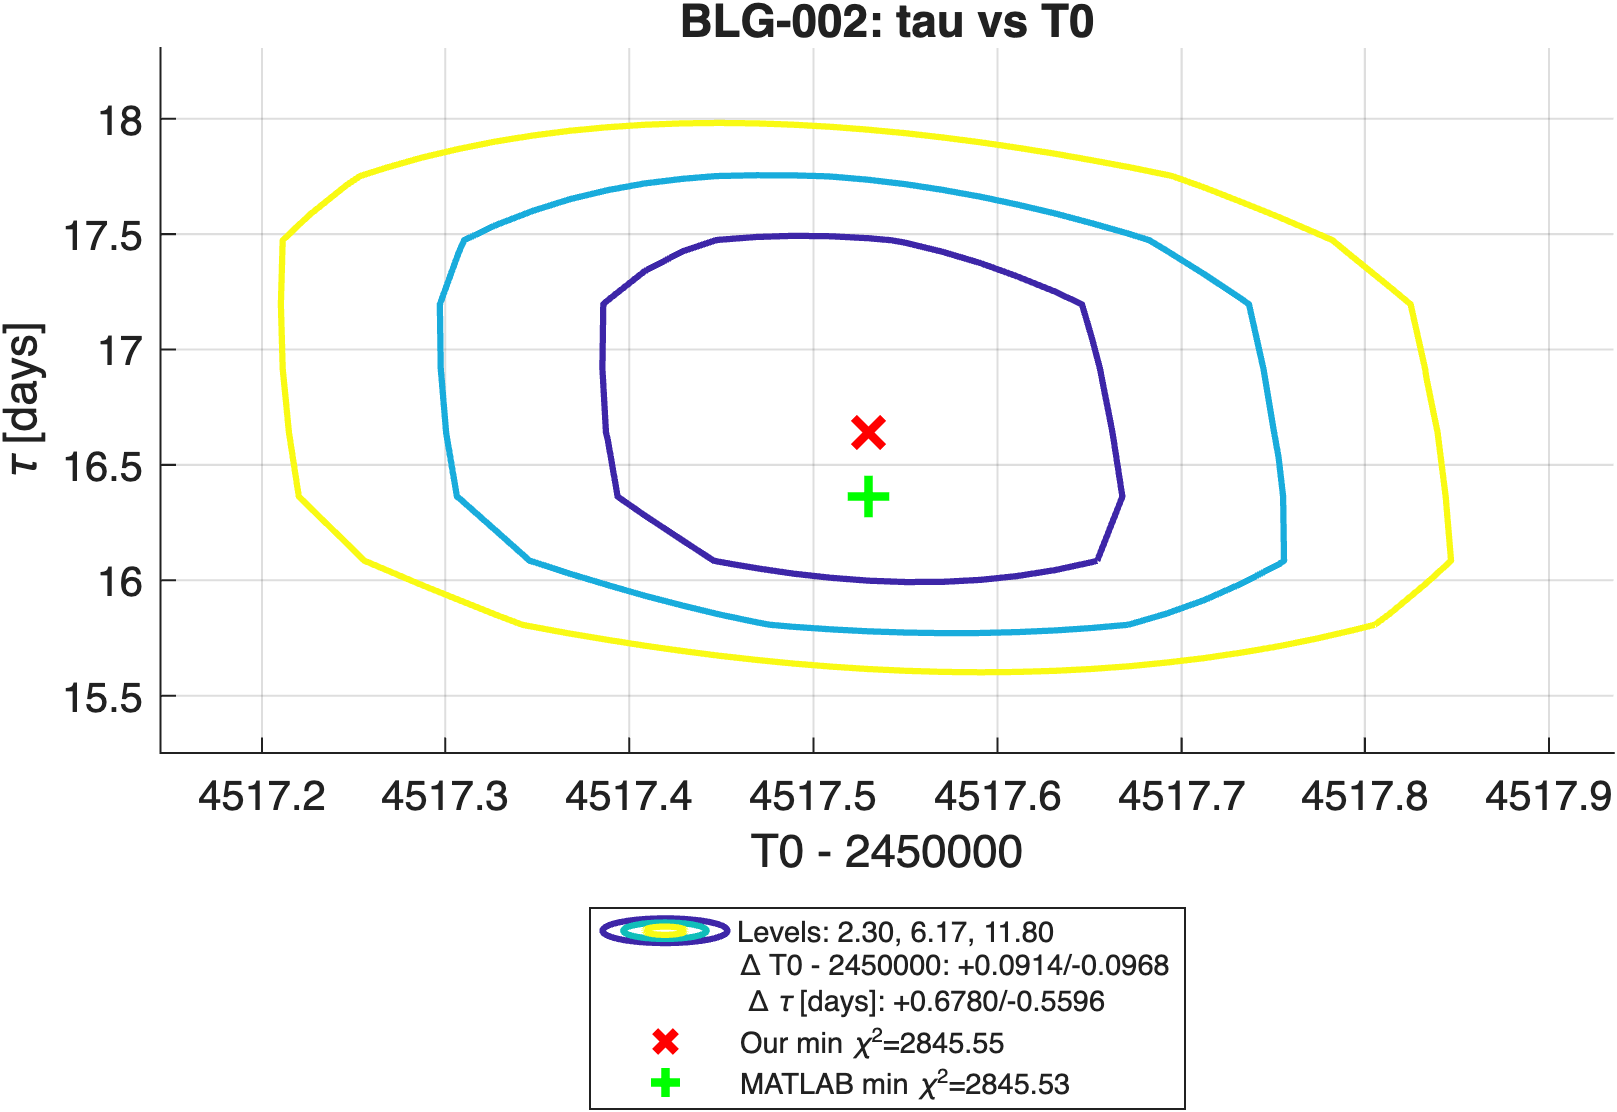
\includegraphics[width=1\linewidth]{Pt5_fig_tau_T0.png}
    \caption{מפת $\Delta\chi^2$ במישור $\tau$-$T_0$}
    \label{fig:part5_tau_T0}
\end{figure}
\begin{figure}[H]
    \centering
    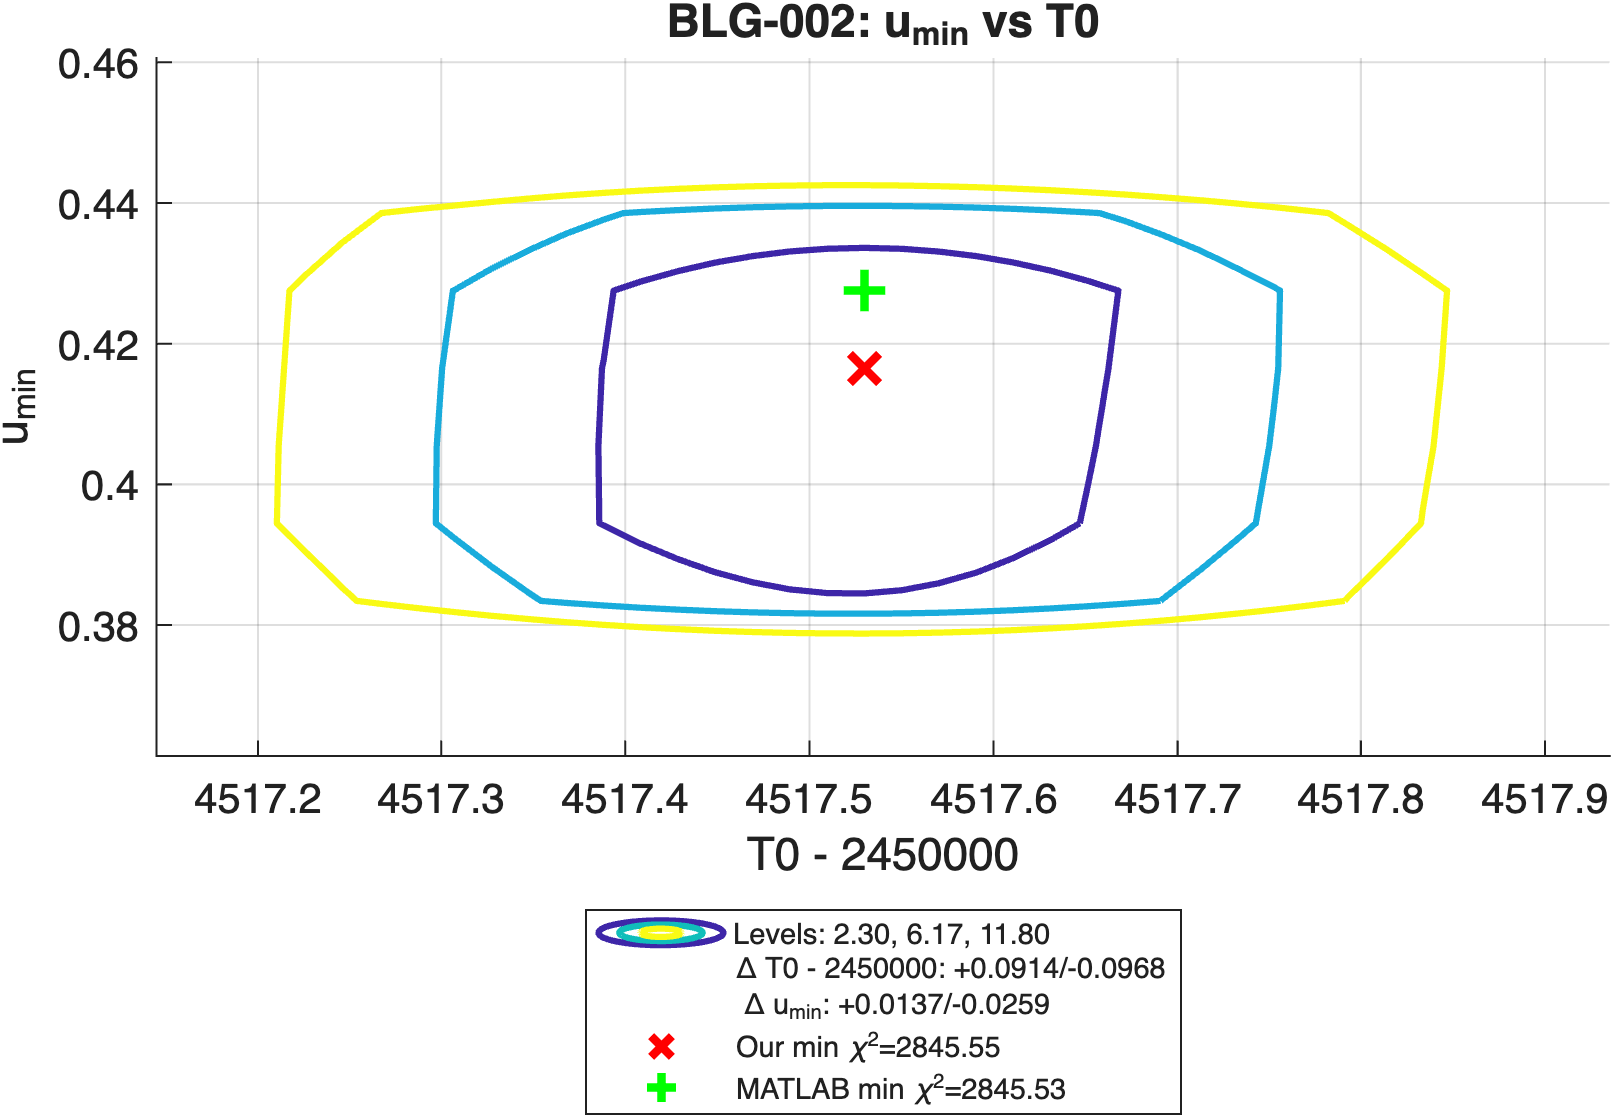
\includegraphics[width=1\linewidth]{Pt5_fig_umin_T0.png}
    \caption{מפת $\Delta\chi^2$ במישור $u_{\min}$-$T_0$}
    \label{fig:part5_umin_T0}
\end{figure}

\begin{figure}[H]
    \centering
    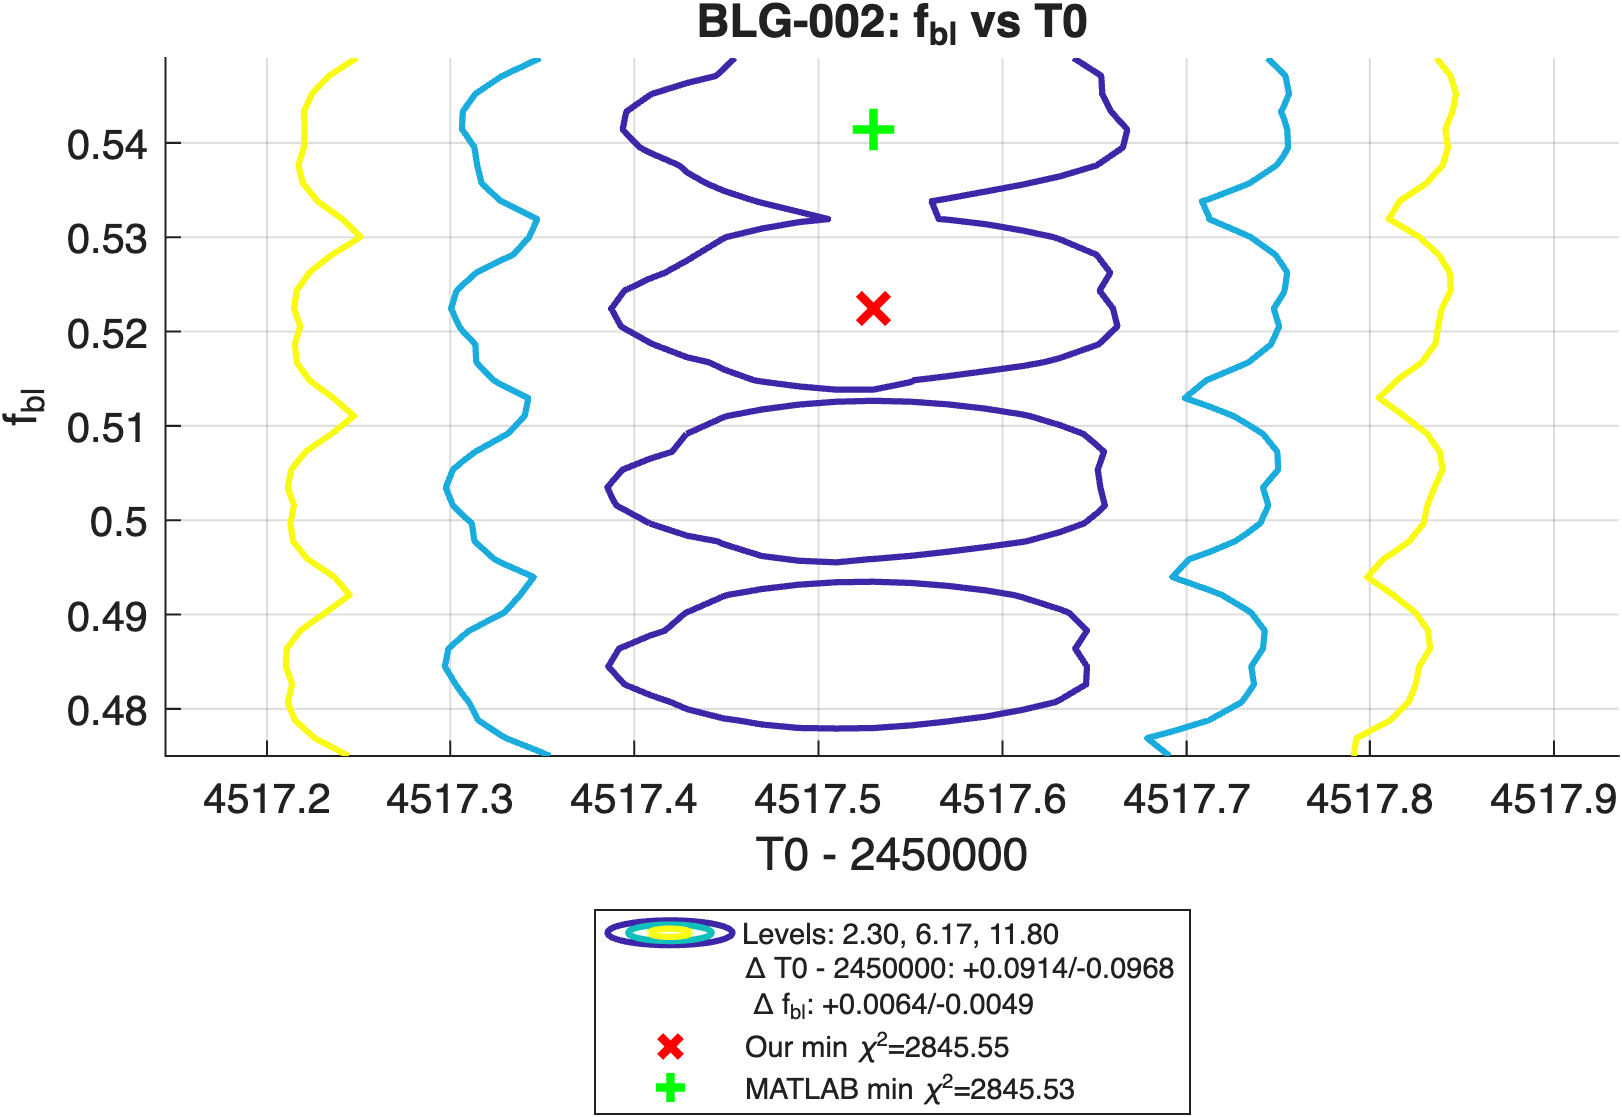
\includegraphics[width=1\linewidth]{Pt5_fig_fbl_T0.png}
    \caption{מפת $\Delta\chi^2$ במישור $f_{bl}$-$T_0$}
    \label{fig:part5_fbl_T0}
\end{figure}


\end{multicols}

\subsection{השוואת שיטות}
\label{app:disscution_compar_methods}


\begin{table}[h]
\centering
\resizebox{\textwidth}{!}{%
\begin{tabular}{|c|c|c|c|c|c|c|c|c|c|c|}
\hline
חלק 
&
פרמטרים
&
\textenglish{$\chi^2_{red}$} 
&
\multicolumn{2}{c|}{\textenglish{$\tau$}} 
&
\multicolumn{2}{c|}{\textenglish{$u_{min}$}} 
&
\multicolumn{2}{c|}{\textenglish{$T_0$}} 
& 
מסה
&
רדיוס איינשטיין
\\
\cline{4-9}
& & & שגיאה יחסית & השוואה ל\textenglish{OGLE} & שגיאה יחסית & השוואה ל\textenglish{OGLE} & שגיאה יחסית & השוואה ל\textenglish{OGLE} & & \\
\hline
א׳ & \textenglish{a,b,c}  & \textenglish{1.0863} & --- & --- & --- & --- &  \textenglish{+0.0000049/-0.0000049\%} & \textenglish{0.0000035\%} & --- & --- \\
ב׳ & \textenglish{$\tau$, $u_{min}$} & \textenglish{1.9267} & \textenglish{+1.19/-1.21\%} & \textenglish{1.519\%} & \textenglish{+0.67/-0.69\%} & \textenglish{0.124\%} & --- & --- & \textenglish{+2.50/-2.53\%} & \textenglish{+1.31/-1.32\%} \\
ג׳ & \textenglish{$\tau$, $u_{min}$, $T_0$} & \textenglish{1.9301} & \textenglish{+1.24/-1.21\%} & \textenglish{1.561\%} & \textenglish{+0.67/-0.69\%} & \textenglish{0.125\%} & \textenglish{+0.0000031/-0.0000034\%} & \textenglish{0.0000016\%} & \textenglish{+2.59/-2.54\%} & \textenglish{+1.35/-1.32\%} \\
\hline
\end{tabular}%
}
\caption{\textenglish{SMC-001}: השוואת שיטות סטטיסטיות}
\end{table}


 
\begin{table}[h]
\centering
\resizebox{\textwidth}{!}{%
\begin{tabular}{|c|c|c|c|c|c|c|c|c|c|c|c|c|}
\hline
חלק
&
פרמטרים
&
\textenglish{$\chi^2_{red}$}
&
\multicolumn{2}{c|}{\textenglish{$\tau$}} 
&
\multicolumn{2}{c|}{\textenglish{$u_{min}$}} 
&
\multicolumn{2}{c|}{\textenglish{$f_{bl}$}} 
&
\multicolumn{2}{c|}{\textenglish{$T_0$}} 
&
מסה
&
רדיוס איינשטיין
\\
\cline{4-11}
& & & שגיאה יחסית & השוואה ל\textenglish{OGLE} & שגיאה יחסית & השוואה ל\textenglish{OGLE} & שגיאה יחסית & השוואה ל\textenglish{OGLE} & שגיאה יחסית & השוואה ל\textenglish{OGLE} & & \\
\hline
ד׳ & \textenglish{$\tau$, $u_{min}$, $f_{bl}$} & \textenglish{2.8140} & \textenglish{+7.25/-5.90\%} & \textenglish{0.652\%} & \textenglish{+11.56/-9.18\%} & \textenglish{1.057\%} & \textenglish{+0.75/-1.59\%} & \textenglish{0.730\%} & --- & --- & \textenglish{+14.11/-11.80\%} & \textenglish{+7.26/-5.90\%} \\
ה׳ & \textenglish{$\tau$, $u_{min}$, $f_{bl}$, $T_0$} & \textenglish{2.1427} & \textenglish{+4.07/-3.36\%} & \textenglish{0.827\%} & \textenglish{+3.29/-6.21\%} & \textenglish{1.341\%} & \textenglish{+1.23/-0.94\%} & \textenglish{2.038\%} & \textenglish{+0.0000037/-0.0000039\%} & \textenglish{0.0000041\%} & \textenglish{+8.15/-6.73\%} & \textenglish{+4.08/-3.70\%} \\
\hline
\end{tabular}%
}
\caption{\textenglish{BLG-002}: השוואת שיטות סטטיסטיות}
\end{table}


\end{document}


